\chapter{Results}
\label{chap:results}




\section{Verification of 5D reconstruction}
The introduction of the fifth dimension was explained in section \ref{chap:SAFT_Augment}. The assignment process of the  voxel value $V_k$ to the voxels in the 4th and 5th dimension was explained in section \ref{sec:index_ident}. The functionality of this process shall be shown in this section. In this example the 4th dimension will relate to the comparison vector from the voxel to the receiver. The 5th dimension is defined as the comparison vector from the voxel to the emitter. During the reconstruction 14 direction vectors were used. 
The configuration of active emitters and receivers is shown in Figure \ref{fig:res:5th_dim_over_4th_aperture}. The green crosses mark the location of all active receivers and the red circles represent the emitters. For this example the first 30235 \acp{ascan} are used which include the first 40 emitters and 1309 receivers. The actual data set includes plenty more \ac{ascan}. Including all of those would lead to a very complex representation so only the first couple thousand were taken. 
As it was explained in section \ref{sec:multimodality} for the reflection imaging technique for one emitter only the relevant receivers are considered during the reconstruction since the others would lower the SNR of the image. Every receiver that lays in a $\pm 120^{\circ}$ angle to the sender normal is included for that particular emitter. This is why in Figure \ref{fig:res:5th_dim_over_4th_aperture} it looks like a slice of receivers is missing in the aperture. They are simply not included in the first set of \acp{ascan}.

\begin{figure}[H]
    \centering
    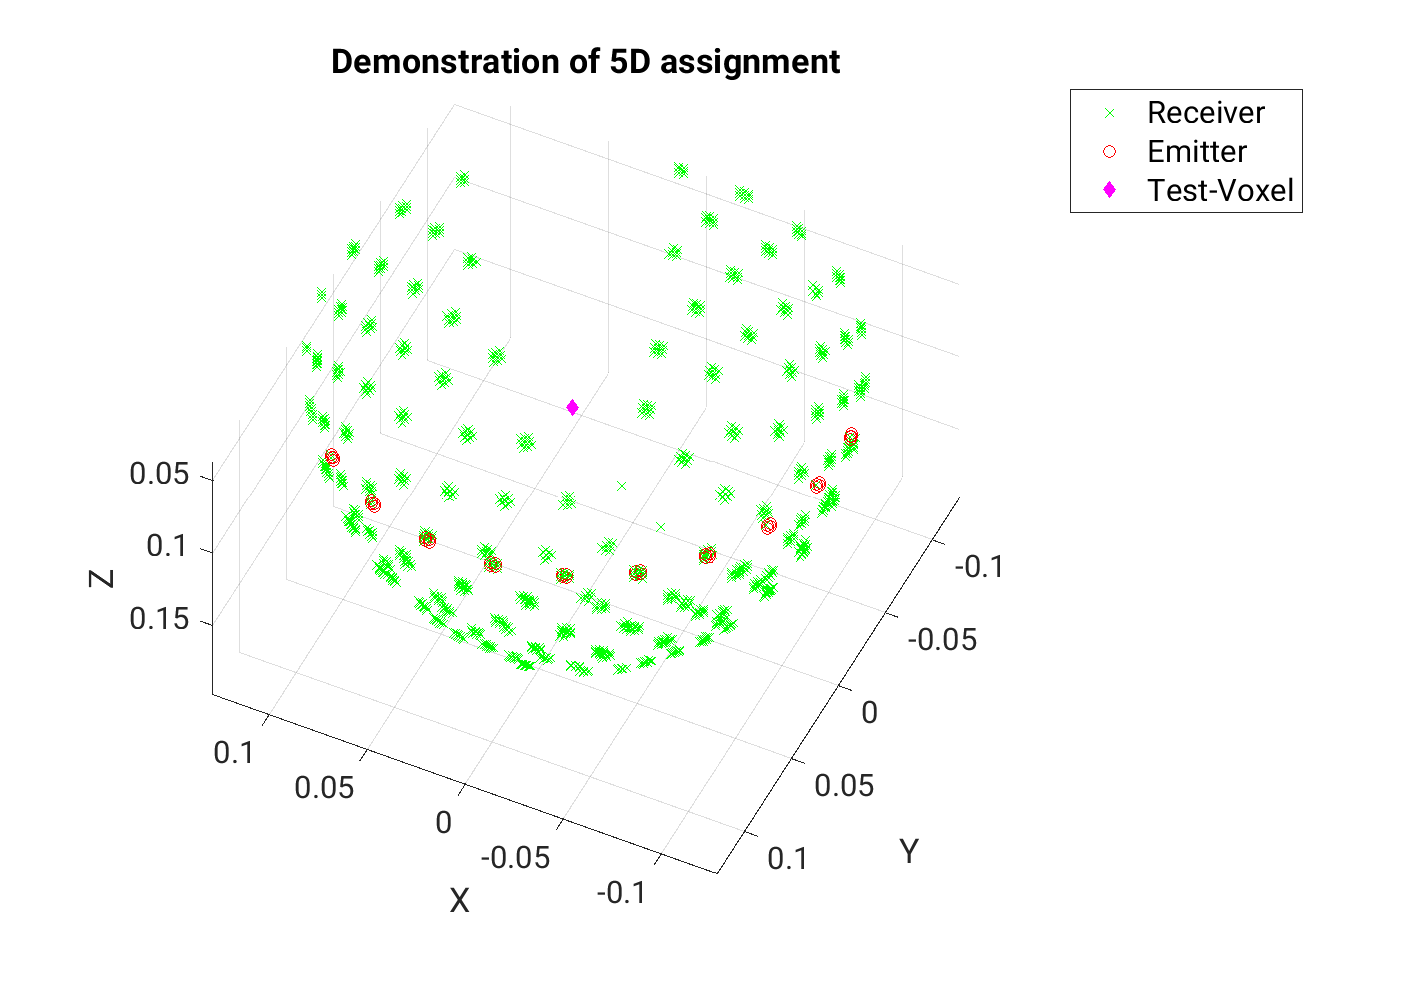
\includegraphics[width=0.89\linewidth]{Graphics/Results/4d_5d/5thDim_over_4thDim_150_150_150_apertur.eps}
    \caption{Configuration of 10 emitting and 145 receiving \ac{tas} and a test voxel in the middle of the aperture. The receivers are shown in green and the emitters as red circles. The units on the axes is given in meter. }
    \label{fig:res:5th_dim_over_4th_aperture}
\end{figure}

 The receiving and emitting transducers are organised as \acp{tas} where each \ac{tas} comprises four emitters and nine receivers. This is why it looks as if all 40 emitters were organised in 10 separate units whereas the 1309 receivers were summarised in 145 green stacks. 
 For this example a test vector is defined arbitrarily in the middle of the aperture at $[150\, , \, 150\, , \, 150]$ and is shown as the pink diamond in Figure \ref{fig:res:5th_dim_over_4th_aperture}. The coordinates of the voxel can be converted into the coordinates system of the \ac{usct} which is given in meters. The test voxel therefore is located at $[0.0047m\, , \, 0.0047m\, , \, 0.0047m]$.

 During the reconstruction the sum of each voxel value $V_k$ from the \ac{saft} for each voxel is saved in the 5D-Volume. The following Figure shows the voxel values for the one test voxel in the centre of the aperture at the position of the pink diamond. Since there are 5 dimensions each dimensions gets assigned a certain amount of voxel values for each combination of dimensions. Every combination of the 4th dimension with the 5th dimension is shown in Figure \ref{fig:res:5th_dim_over_4th_result}.
 
 
\begin{figure}[H]
    \centering
    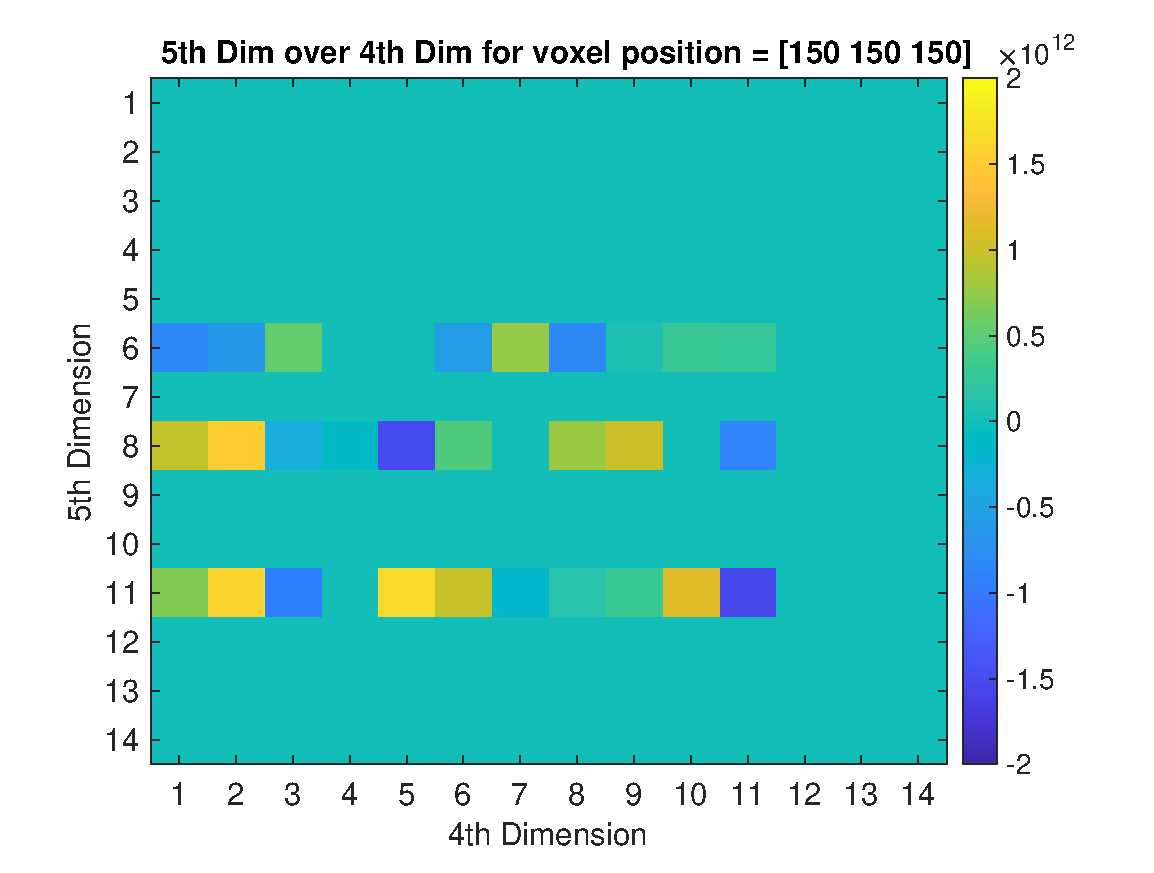
\includegraphics[width=0.89\linewidth]{Graphics/Results/4d_5d/5thDim_over_4thDim_150_150_150.eps}
    \caption{Resulting voxel values $V_k$ of the five dimensional reconstruction. The 4th dimension relates to the voxel-receiver-vector. The 5th dimension represents the directional information for the voxel-emitter-vector.}
    \label{fig:res:5th_dim_over_4th_result}
\end{figure}

To understand this image one might want to remember the example of the Rubik's cubes from section \ref{chap:SAFT_Augment}. In particular the 5D example in Figure \ref{5D_rubics} should help to understand the illustration in Figure \ref{fig:res:5th_dim_over_4th_result}. For the conservation of the directional information each 3D image volume that was represented by a Rubik's cube was repeated into the 4th dimension as many times as there are direction vectors available. Ultimately the 4th dimension then was repeated into the 5th dimension which yielded a $M \times M$ matrix of Rubik's cubes for $M$ direction vectors. In the previous example there were only four direction vectors. So, this resulted in $4 \times 4 = 16$ Rubik's cubes. In this example here we work with 14 direction vectors which would lead to a $14 \times 14$ matrix with a total of 196 Rubik's cubes. These 196 Rubik's cubes practically are shown in Figure \ref{fig:res:5th_dim_over_4th_result} but not as whole but always the value of the same voxel in each cube. To be precise the voxel value for voxel $[150\, , \, 150\, , \, 150]$ was taken from each of the 196 Rubik's cubes and placed in the 5D-over-4D-representation in the aforementioned figure.
Every value that can be found in same row of the matrix was recorded by the same emitter. Likewise, every value in the same column belongs to the same receiver. The distribution of value becomes clear if one takes a look at the emitter-receiver-configuration from Figure \ref{fig:res:5th_dim_over_4th_aperture} above with every direction vector and every decision cone. This is shown in the following Figure for some of the 14 cones:


\begin{figure}[H]
     \centering
     \begin{subfigure}[b]{0.49\textwidth}
         \centering
        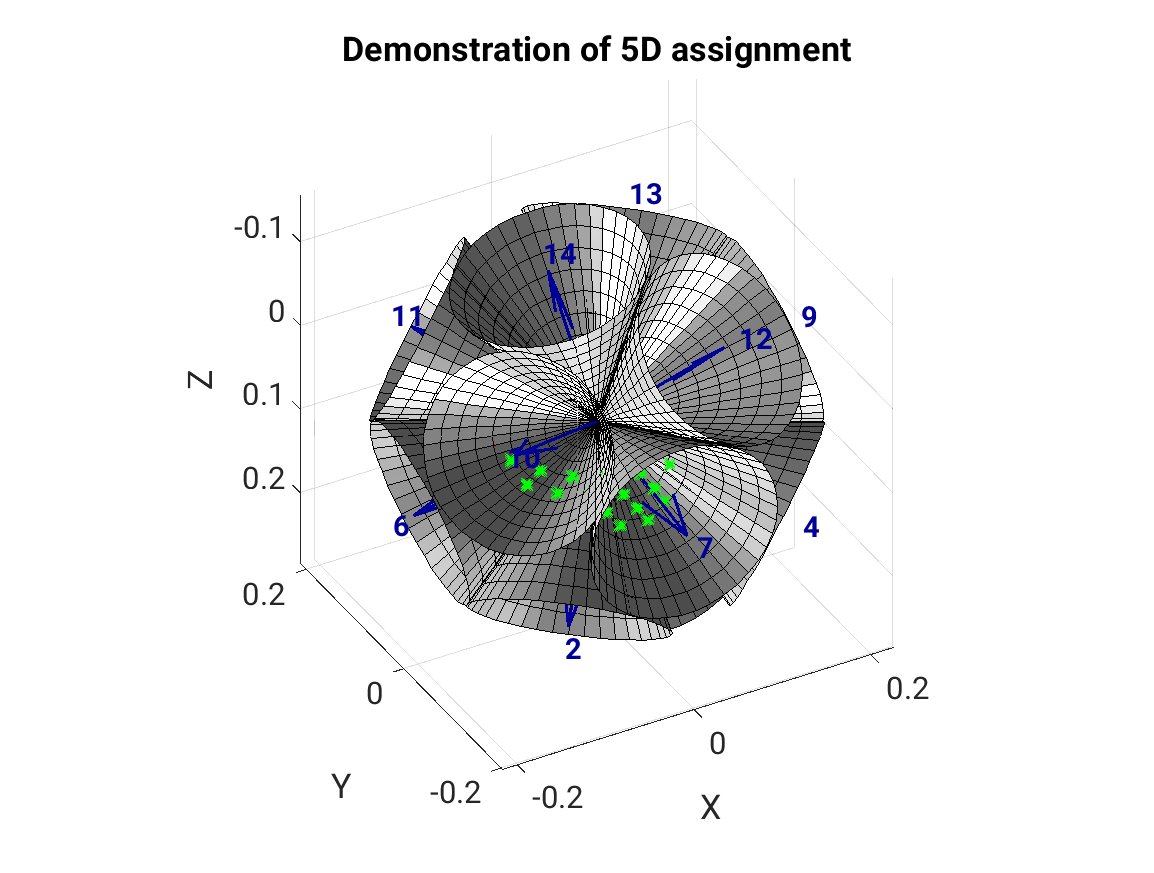
\includegraphics[width=1.12\linewidth,right]{Graphics/Results/4d_5d/5thDim_over_4thDim_150_150_150_cones_10_center.eps}
         \caption{Cone 10}
         \label{fig:res:5th_4th_cones10}
     \end{subfigure}
     \hfill
     \begin{subfigure}[b]{0.49\textwidth}
         \centering
         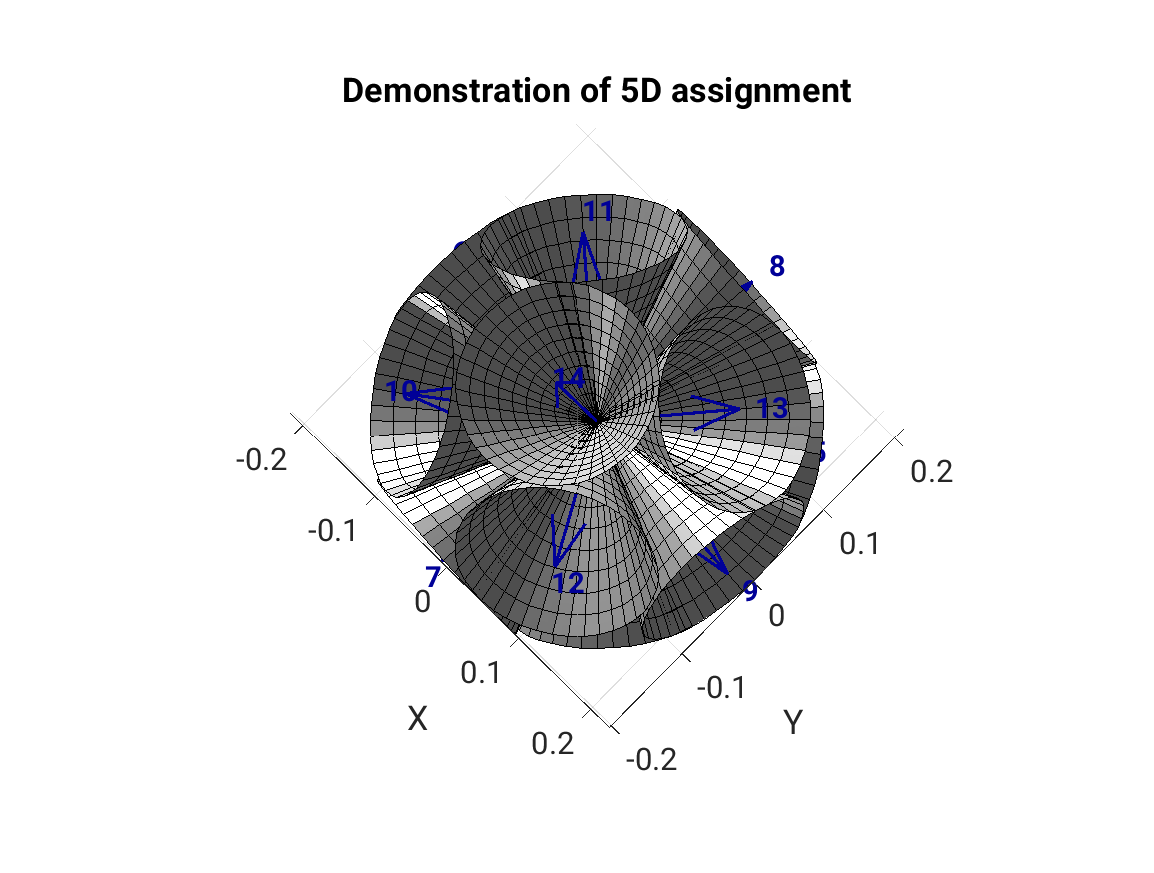
\includegraphics[width=1.3\textwidth,right]{Graphics/Results/4d_5d/5thDim_over_4thDim_150_150_150_cones_14_center.eps}
         \caption{Cone 14}
         \label{fig:res:5th_4th_cones14}
     \end{subfigure}
     \hfill
     \begin{subfigure}[b]{0.49\textwidth}
         \centering
         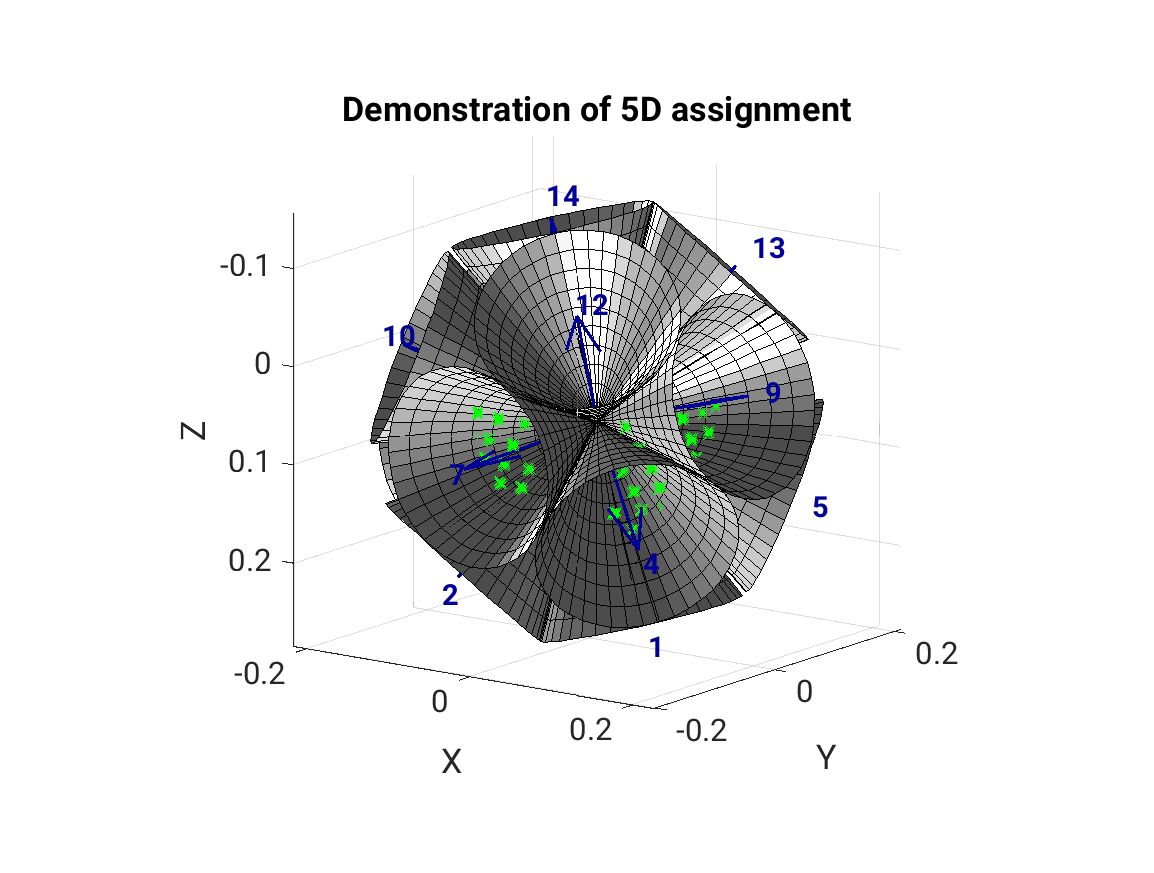
\includegraphics[width=1.3\textwidth,right]{Graphics/Results/4d_5d/5thDim_over_4thDim_150_150_150_cones_7_9_center.eps}
         \caption{Cone 12}
         \label{fig:res:5th_4th_cones12}
     \end{subfigure}
     \hfill
     \begin{subfigure}[b]{0.49\textwidth}
         \centering
         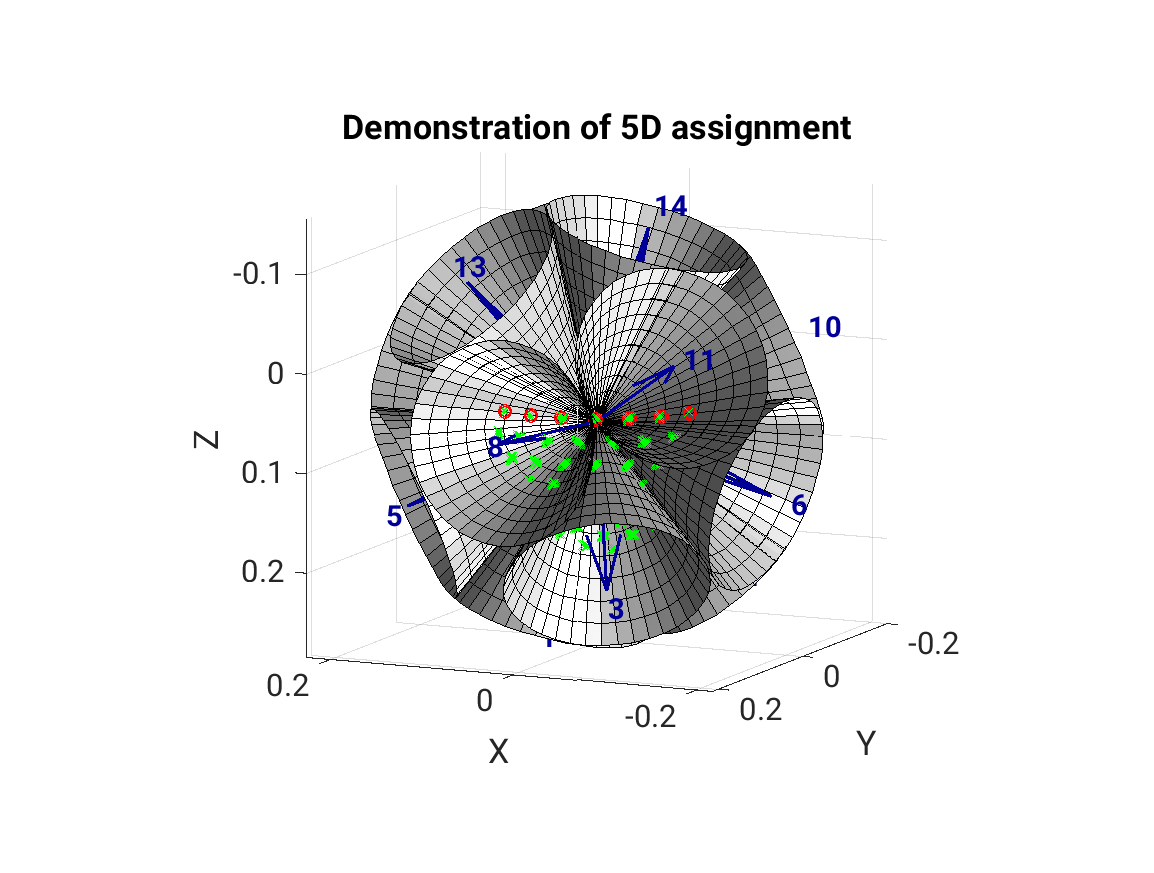
\includegraphics[width=1.3\textwidth,right]{Graphics/Results/4d_5d/5thDim_over_4thDim_150_150_150_cones_8_11_center.eps}
         \caption{Cone 11}
         \label{fig:res:5th_4th_cones11}
     \end{subfigure}
     \hfill
     \begin{subfigure}[b]{0.49\textwidth}
         \centering
         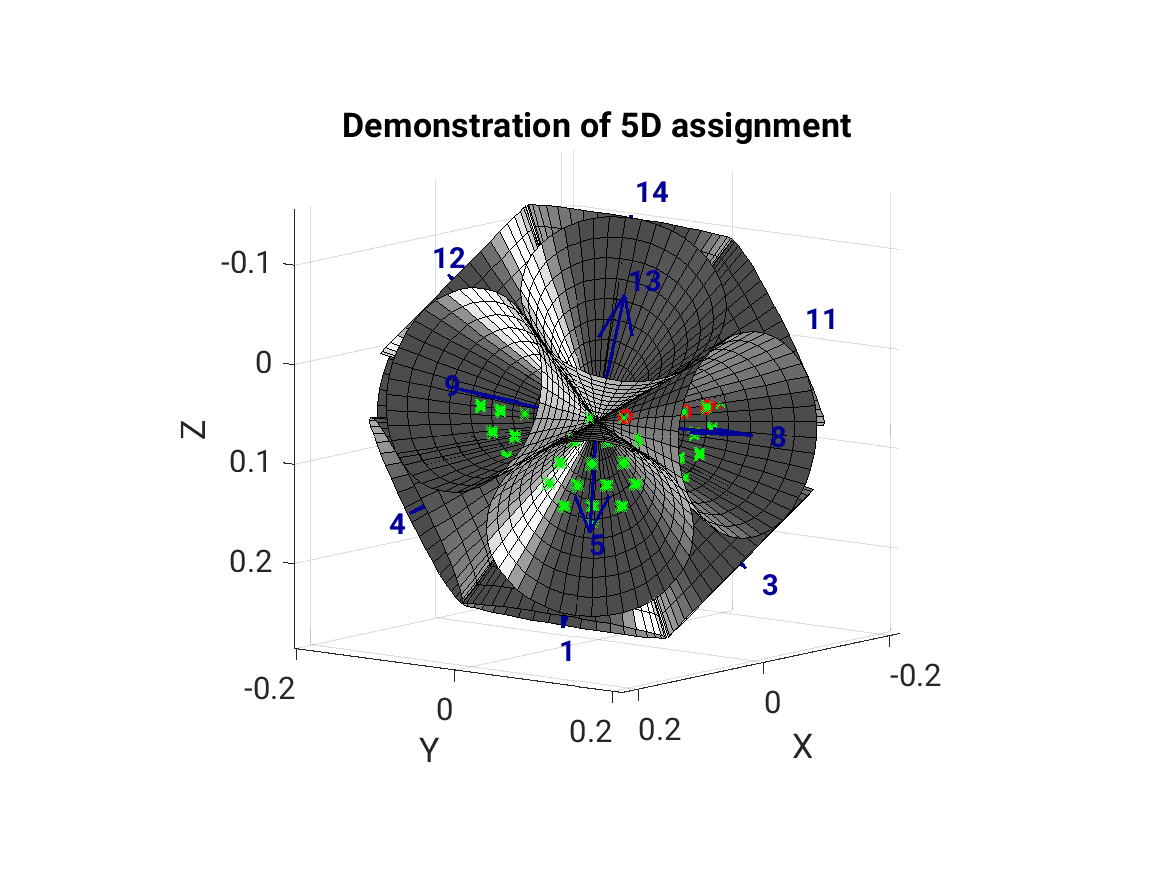
\includegraphics[width=1.3\textwidth,right]{Graphics/Results/4d_5d/5thDim_over_4thDim_150_150_150_cones_9_8_center.eps}
         \caption{Cone 5}
         \label{fig:res:5th_4th_cones5}
     \end{subfigure}
        \caption{The emitter-receiver-configuration of Figure \ref{fig:res:5th_dim_over_4th_aperture} with added direction vectors and decision cones. The origin of each cone is located at the position of the test voxel $[150\, , \, 150\, , \, 150]$. }
        \label{fig:res:5th_4th_cones}
\end{figure}

To connect the results shown in Figure \ref{fig:res:5th_dim_over_4th_result} with the cone images in Figure \ref{fig:res:5th_4th_cones} we start with looking at the red dots in the 5d-over-4d image. These red dots are representing the emitters which were active during the first set of \acp{ascan}. When the \ac{saft} is executed a voxel value $V_k$ is calculated. For this voxel value and its corresponding voxel the comparison vector from the voxel to the emitter is constructed. This voxel-emitter-comparison-vector then is assigned to the direction vectors. This is done by checking in what cone the comparison vector lands. In Figure \ref{fig:res:5th_4th_cones} for every red dot that is visible in one of the cones this means that there is a comparison vector from the test voxel $[150\, , \, 150\, , \, 150]$ to that particular emitter and it is assigned to the cone where the red emitter is visible in. In this example the following cones contain red dots: 6, 8 and 11. The results in Figure \ref{fig:res:5th_dim_over_4th_result} show, that the only the rows for 6, 8 and 11 are occupied. All other rows are empty. This coincides with the assumption that the 5th dimension relates to the voxel-emitter-comparison-vector and that the emitters are only assigned to three direction vectors. 
For the receivers, which are plotted in green, the comparison vectors from the voxel to the receiver are relevant and the data can be found in the fourth dimension. This is why in Figure \ref{fig:res:5th_dim_over_4th_result} only the columns are occupied for that direction vectors were assigned to the green receiver dots. Figure \ref{fig:res:5th_4th_cones14} shows an example of cones where neither a red emitter nor a green receiver is located in. The empty cones in this case are 12, 13 and 14. These are the cones that point toward the opening of the aperture where no transducers are located. Therefore, it is no surprise that no data is recorded from there. In the 5D-over-4D representation of the voxel values these are the dimensions where neither the column nor the rows are occupied.



\section{Variance imaging}


Since the final image of the reconstruction contains data in 5 dimensions a method had to be found to extract the data of the 5 dimensions and put it back into a 3D image. One approach for that was to plot the variance image of the measurement volume. 
In Figure \ref{fig:res:5th_dim_over_4th_result} the 5D-over-4D-representation for one voxel location was introduced. It shows each value of a certain voxel at the same location in each of the sub-volumes. The size of the 5D-over-4D-representation depends on the number of direction vectors that were used.   







\section{Implementation of the code}

\section{Comparison of orthogonality threshold method and angle sorting method}

In section \ref{sec:index_ident} two methods for the assignment of comparison vectors to the right direction vector were explained. It was also mentioned that both methods have different decision regions for the direction vectors. The influence of these differences shown in this section. In the following all images were created using 25 direction vectors and with the added 4th dimension which stores the information about the voxel-receiver relation. The reason for not also including the 5th dimension was to keep the computation time as small as possible and still being able indicate the differences in the resulting images. The following Figure \ref{fig:res:slice_diff_bubble_ortho_image} shows a side by side comparison of the reflection image for both assignment methods. From the 4D image the following configuration was depicted: $[:\,,\,:\,,\,166\,,\,3]$. In other words the following images are from the 3rd direction vector and the 166th slice in the z-dimension. The outline of the olive is recognisable but the overall contrast is not that high. The reason for that is, that for these images the available \acp{ascan} only were partially used. Furthermore, all the \acp{ascan} that actually were used are distributed over 25 sub-volumes in the 4th dimension. With more input data the overall contrast could be increased by a large margin.


\begin{figure}[H]
     \centering
     \begin{subfigure}[b]{0.49\textwidth}
         \centering
        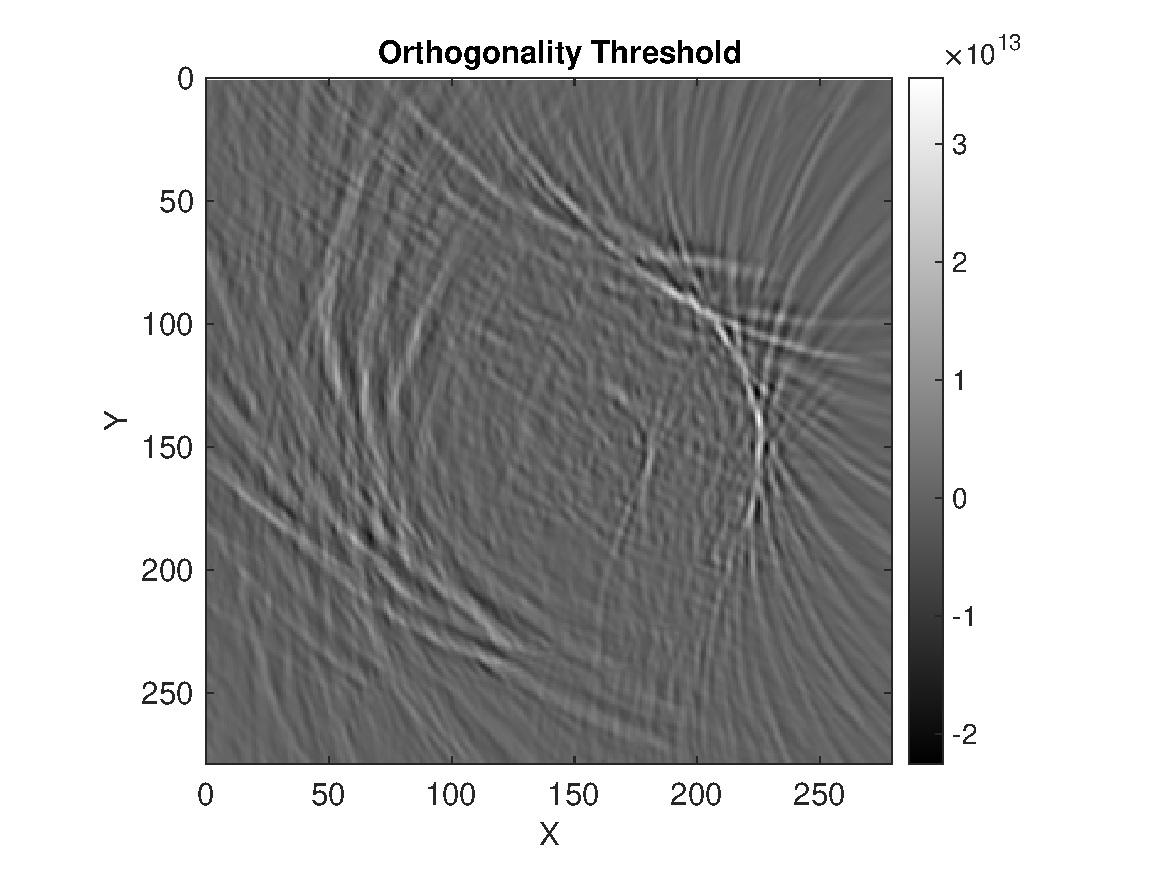
\includegraphics[width=1.12\linewidth,right]{Graphics/Results/Diff_angle_sort_orthogonality/diff_ortho_bubble_slice_166_3_ortho.eps}
         \caption{Orthogonality threshold method.}
         \label{fig:res:slice_diff_bubble_ortho_image_ortho}
     \end{subfigure}
     \hfill
     \begin{subfigure}[b]{0.49\textwidth}
         \centering
         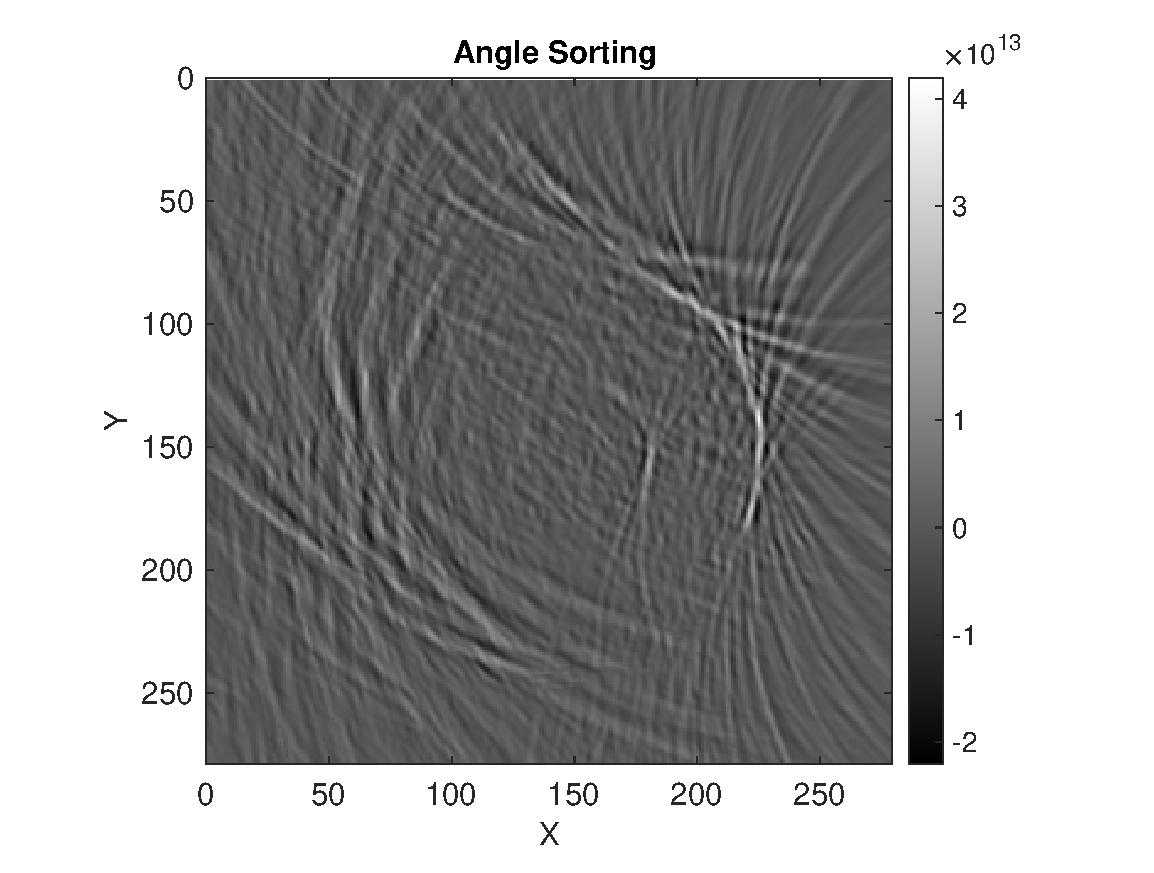
\includegraphics[width=1.12\textwidth,right]{Graphics/Results/Diff_angle_sort_orthogonality/diff_ortho_bubble_slice_166_3_sort.eps}
         \caption{Angle sorting method.}
         \label{fig:res:slice_diff_bubble_ortho_imagebubble}
     \end{subfigure}
        \caption{Side by side comparison of the resulting images for both methods. 25 direction vectors in total were used. The images are shown for the 3rd direction vector and the 166th slice in the z-dimension.}
        \label{fig:res:slice_diff_bubble_ortho_image}
\end{figure}

Figure \ref{fig:res:slice_diff_bubble_ortho_imagebubble} on the right shows a slightly higher contrast than its counterpart on the left. The reason for that is that the Angle Sorting method of section \ref{chap:angle_sorting} assigns every available \ac{ascan} to a direction vector whereas the Orthogonality Threshold method discards every \ac{ascan} for which the comparison vector lay between the cones. 

\bigskip

In the following image the two methods shall be compared for one voxel in each of the 25 volumes in the 4th dimension. This representation is similar to the one in Figure \ref{fig:res:5th_dim_over_4th_result} where the 5th dimension was plotted over the 4th dimension. Since there is not 5th dimension this time only the 4th dimension is plotted. For this representation there is also the analogy of the Rubik's cubes in figure \ref{4D_rubics}. Instead of the four Rubik's Cubes we now have 25 and for each of those cubes the voxel value at the the coordinates $[150\, , \, 150\, , \, 166]$ is displayed. For the direction vectors 22 to 25 no or only very few values are shown. The reason for that again is that those direction vectors are pointing out of the aperture and there are no receivers that could detect or emit a signal. 


\begin{figure}[H]
     \centering
     \begin{subfigure}[b]{0.85\textwidth}
         \centering
        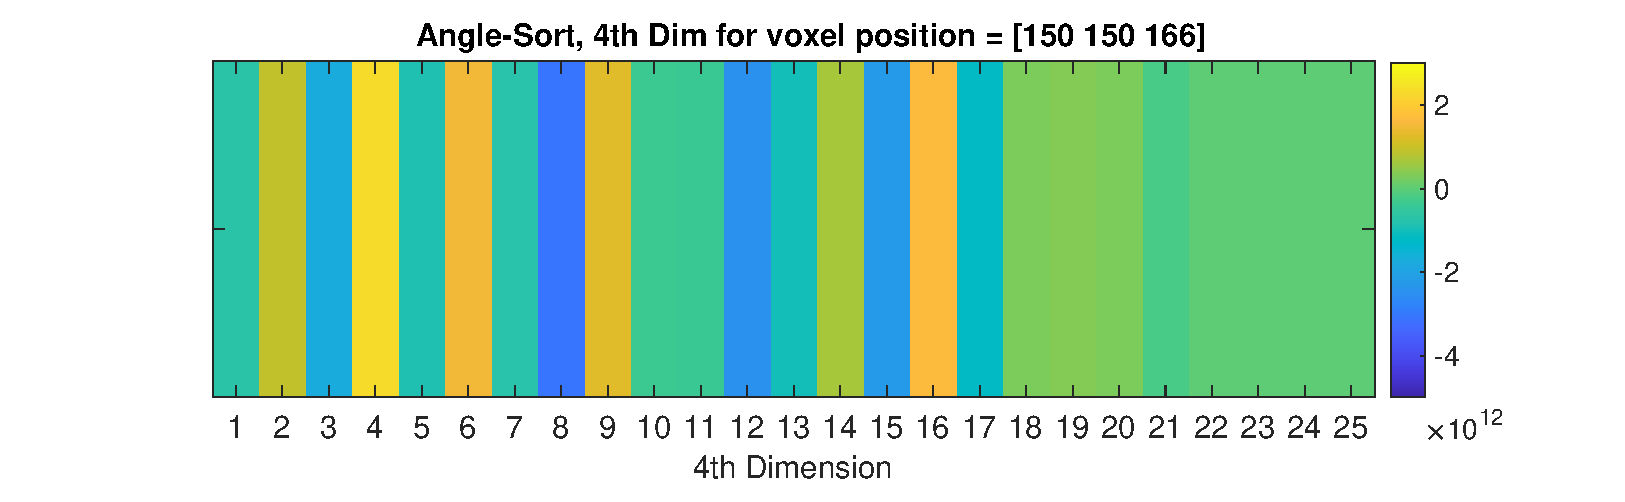
\includegraphics[width=1.12\linewidth,right]{Graphics/Results/Diff_angle_sort_orthogonality/diff_ortho_bubble_25dim_150150150_ortho.eps}
         \caption{Orthogonality threshold method.}
         \label{fig:res:25_voxel_values_diff_bubble_ortho_image_ortho}
     \end{subfigure}
     \hfill
     \begin{subfigure}[b]{0.85\textwidth}
         \centering
         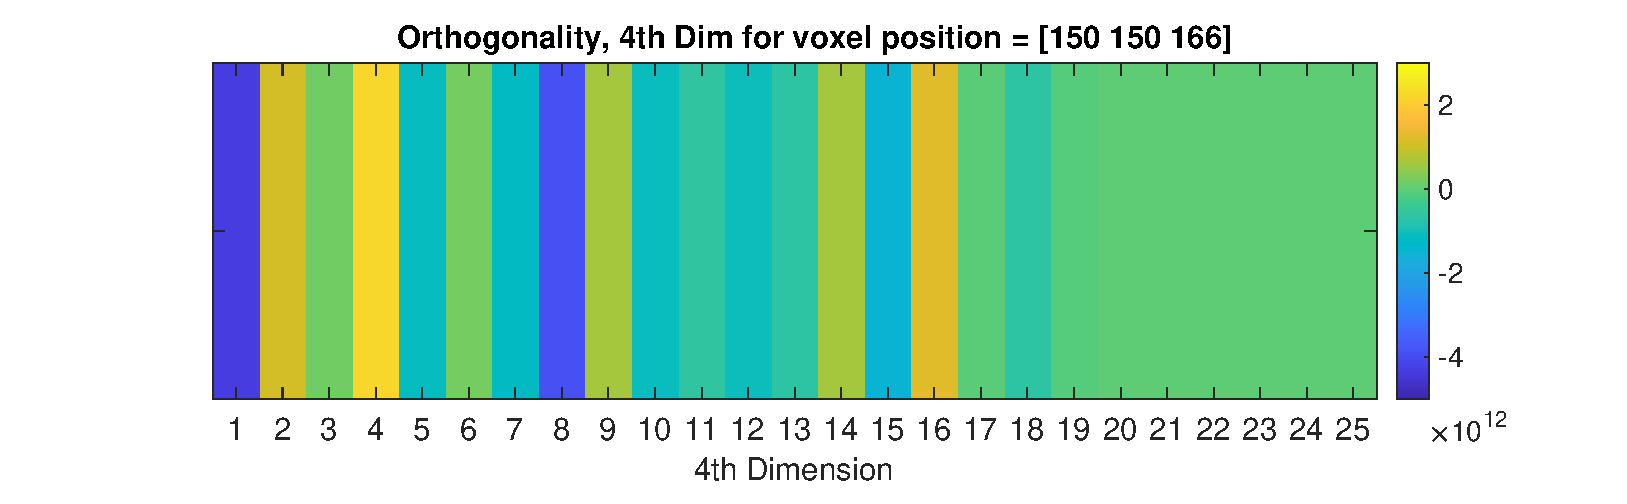
\includegraphics[width=1.12\textwidth,right]{Graphics/Results/Diff_angle_sort_orthogonality/diff_ortho_bubble_25dim_150150150_sort.eps}
         \caption{Angle sorting method.}
         \label{fig:res:25_voxel_values_diff_bubble_ortho_image_bubble}
     \end{subfigure}
        \caption{Comparison of each voxel value for each of the 25 direction vectors.}
        \label{fig:res:25_voxel_values_diff_bubble_ortho_image}
\end{figure}

The overall structure of array of voxel values for the both methods looks similar. Still, there are some differences. For example for the 1st direction vector. The voxel value for the Orthogonality Threshold method was $-4.3171 \times 10^{12}$  where as the voxel value for the angle sorting method was $-7.1738\times10^{11}$ so with the angle sorting value being approximately six times higher. For the comparison of the other voxels Figure \ref{fig:Voxel_value_25} shows each voxel value for the total of 25 direction vectors. The red line shows the voxel values which where yielded by the Orthogonality Threshold approach. The blue graph belongs to the Angle Sorting method. In most points the blue line lays above the red line. This corresponds to the assumption that the Orthogonality Threshold method does not consider every \ac{ascan} and therefore this method yields images with an overall lower contrast. In some cases the lines are congruent, in some they differ completely.  




\begin{figure}[H]
    \centering
    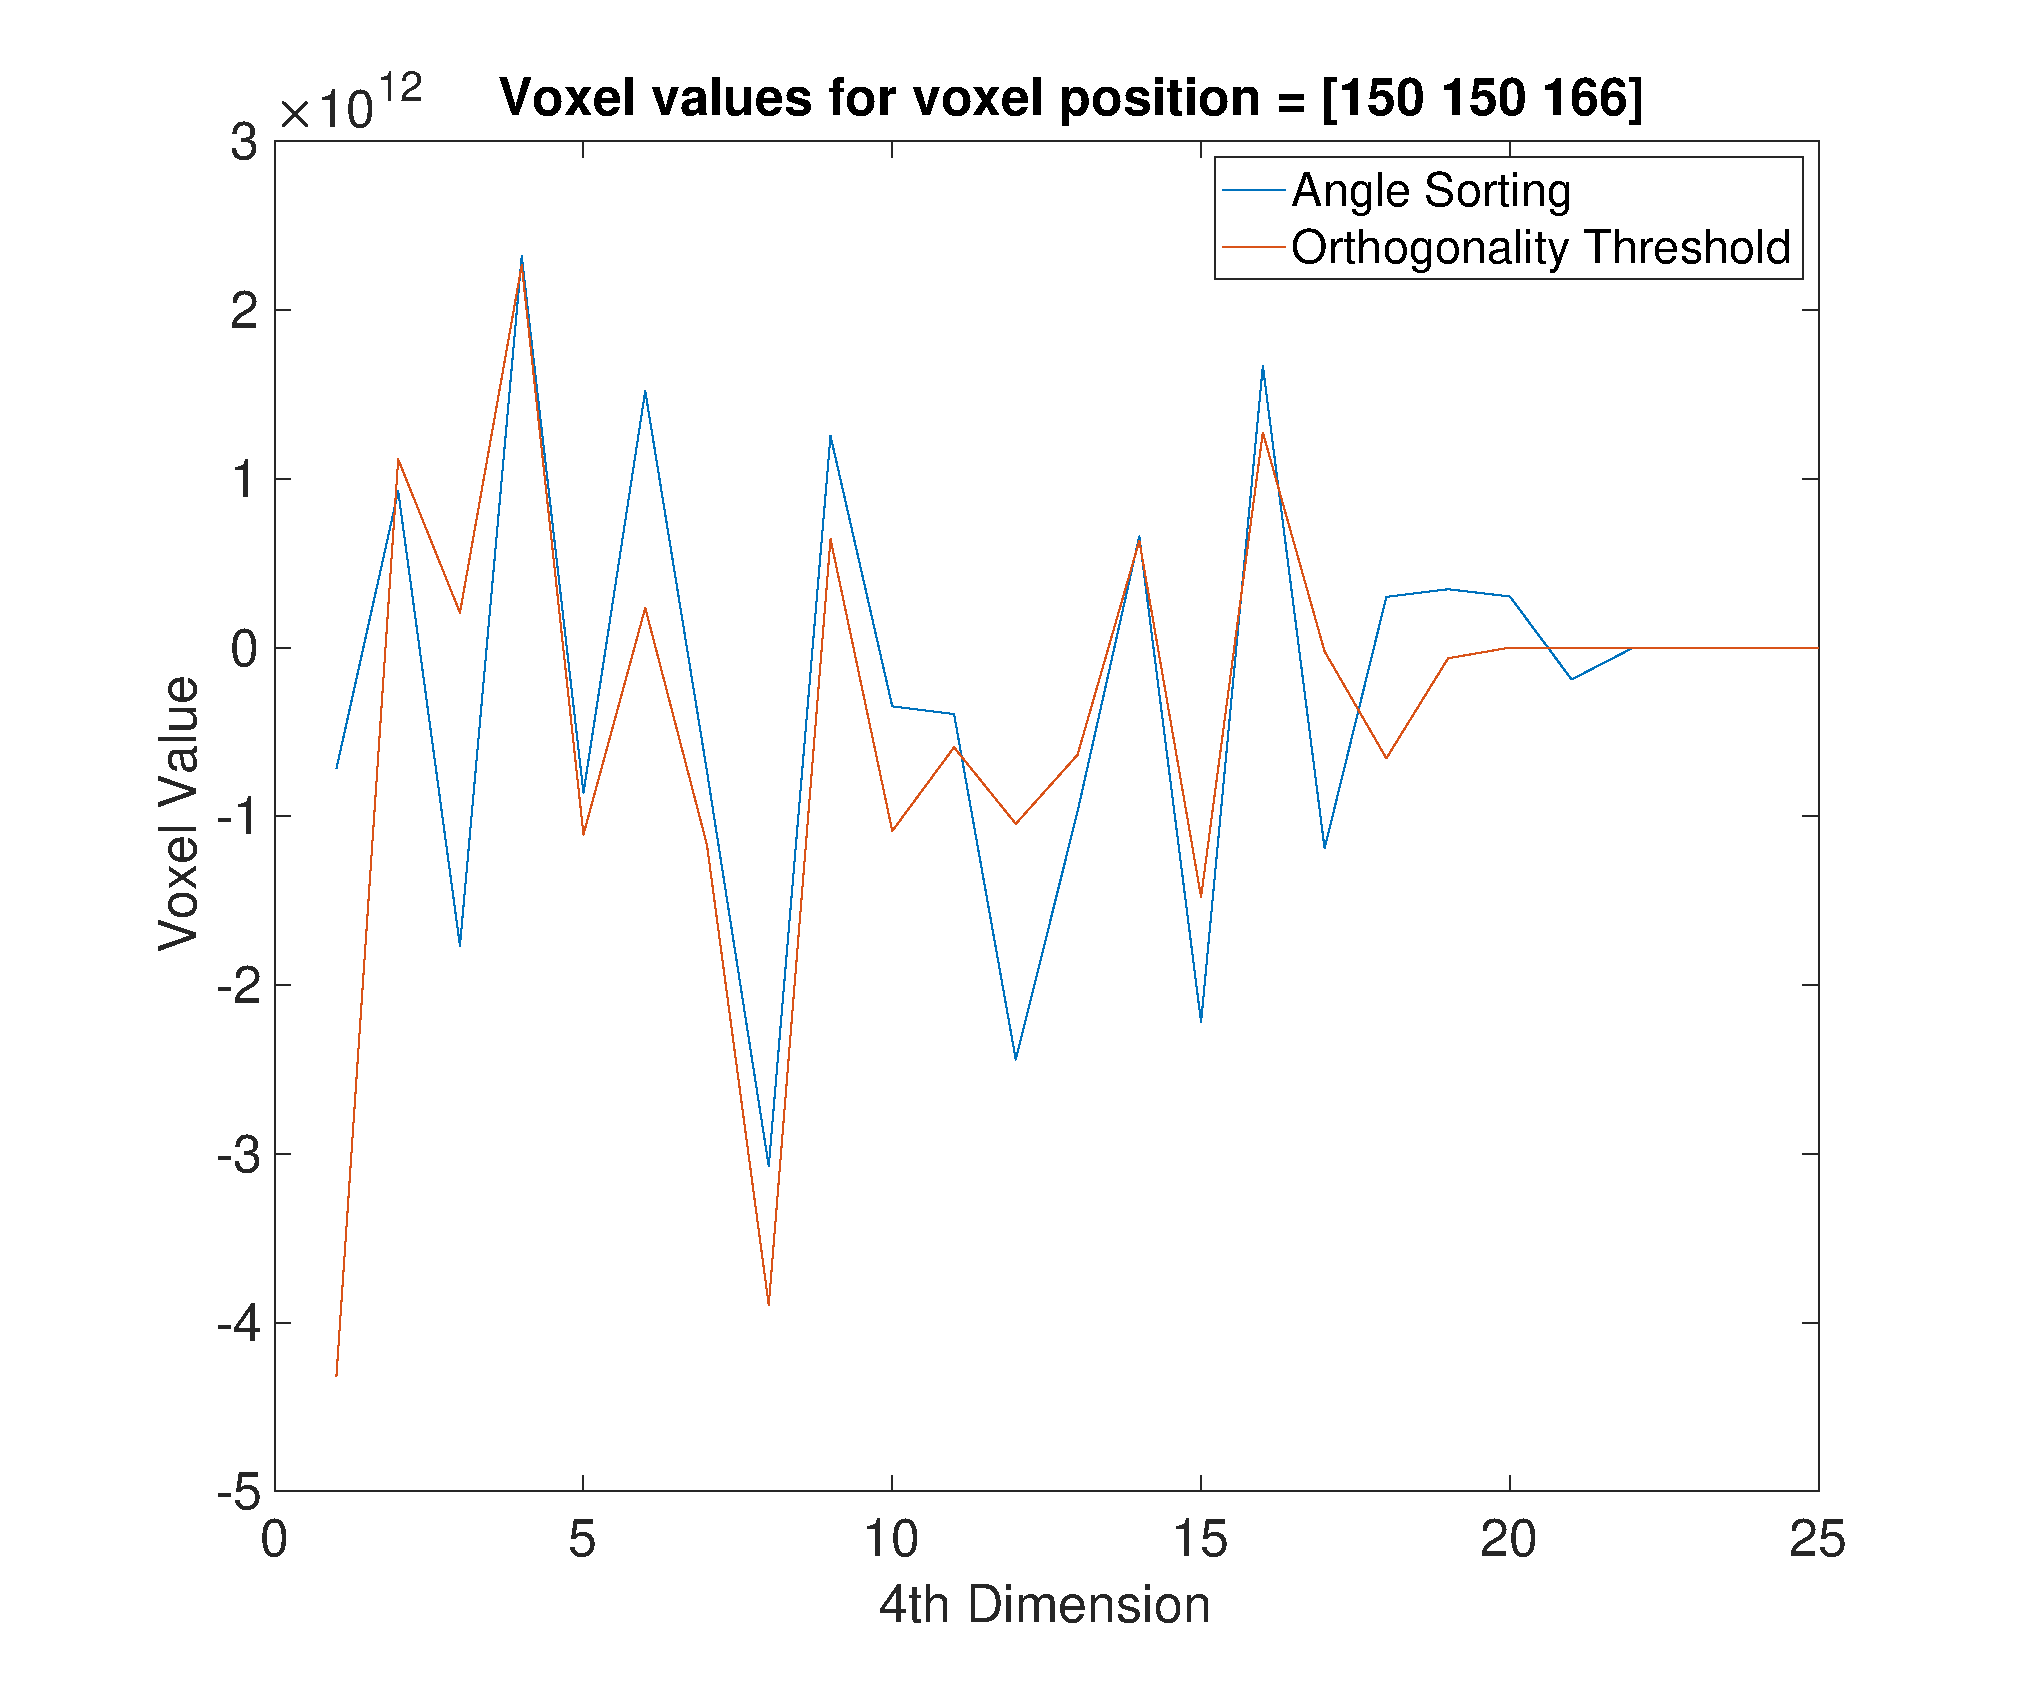
\includegraphics[width=0.82\linewidth]{Graphics/Results/Diff_angle_sort_orthogonality/diff_ortho_bubble_voxelvalues_150150166_sort.eps}
    \caption{Each voxel value of Figure \ref{fig:res:25_voxel_values_diff_bubble_ortho_image} as diagram. The blue graph belongs to the Angle Sorting Method and the red graph to the Orthogonality Threshold. }
    \label{fig:Voxel_value_25}
\end{figure}


To make an assessment about how big the influence of the reduced contrast of the Orthogonality Frequency method really is the reconstructed 4D images are both reduced to a 3D image. For each of the 25 sub-volumes the same voxel position is considered. This leads to 25 voxel values for one particular voxel in each volume. The mean of those 25 voxel values is calculated and written back into the coordinates of the particular voxel. This is repeated for every voxel there is. The final images are shown in the following Figure:


\begin{figure}[H]
     \centering
     \begin{subfigure}[b]{0.49\textwidth}
         \centering
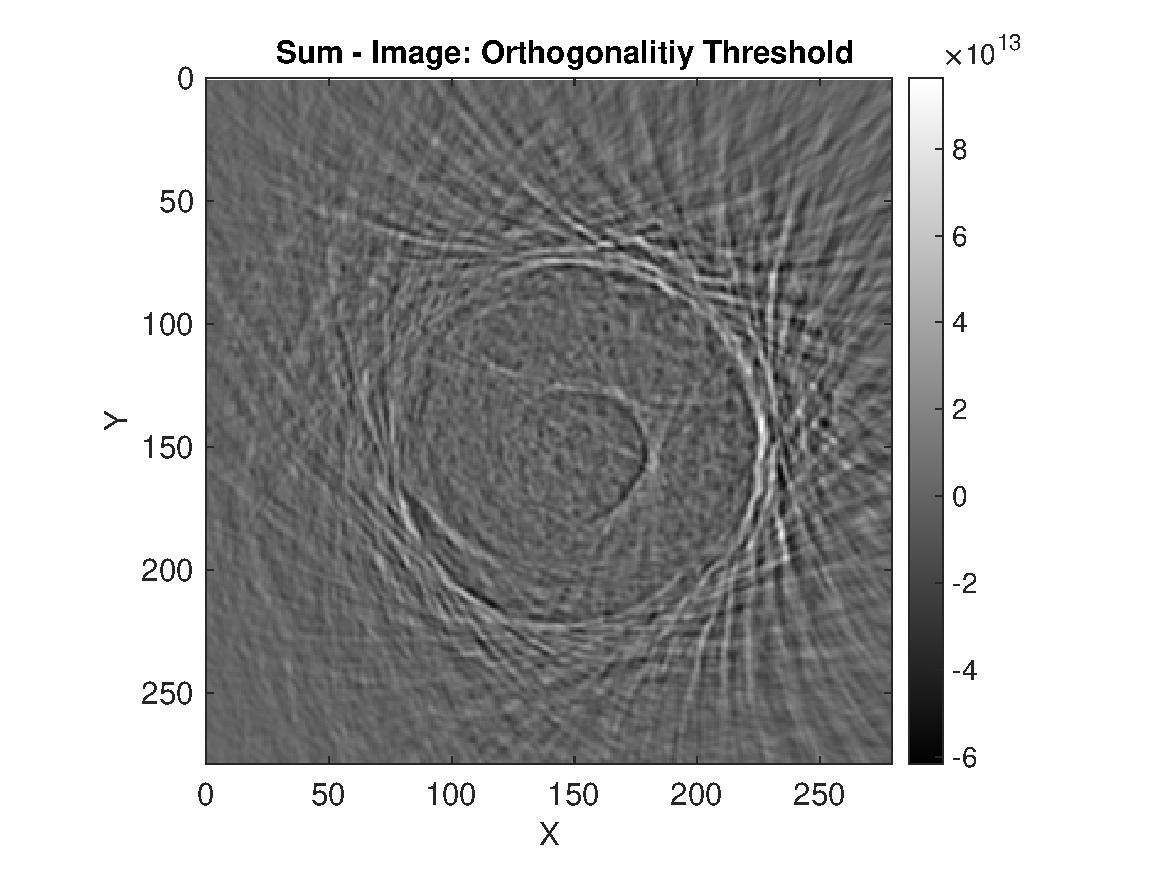
\includegraphics[width=1.12\linewidth,right]{Graphics/Results/Diff_angle_sort_orthogonality/diff_ortho_bubble_sumImmage_ortho.eps}
         \caption{Orthogonality Threshold method.}
         \label{fig:res:summareized_bubble_ortho_image_ortho}
     \end{subfigure}
     \hfill
     \begin{subfigure}[b]{0.49\textwidth}
         \centering
         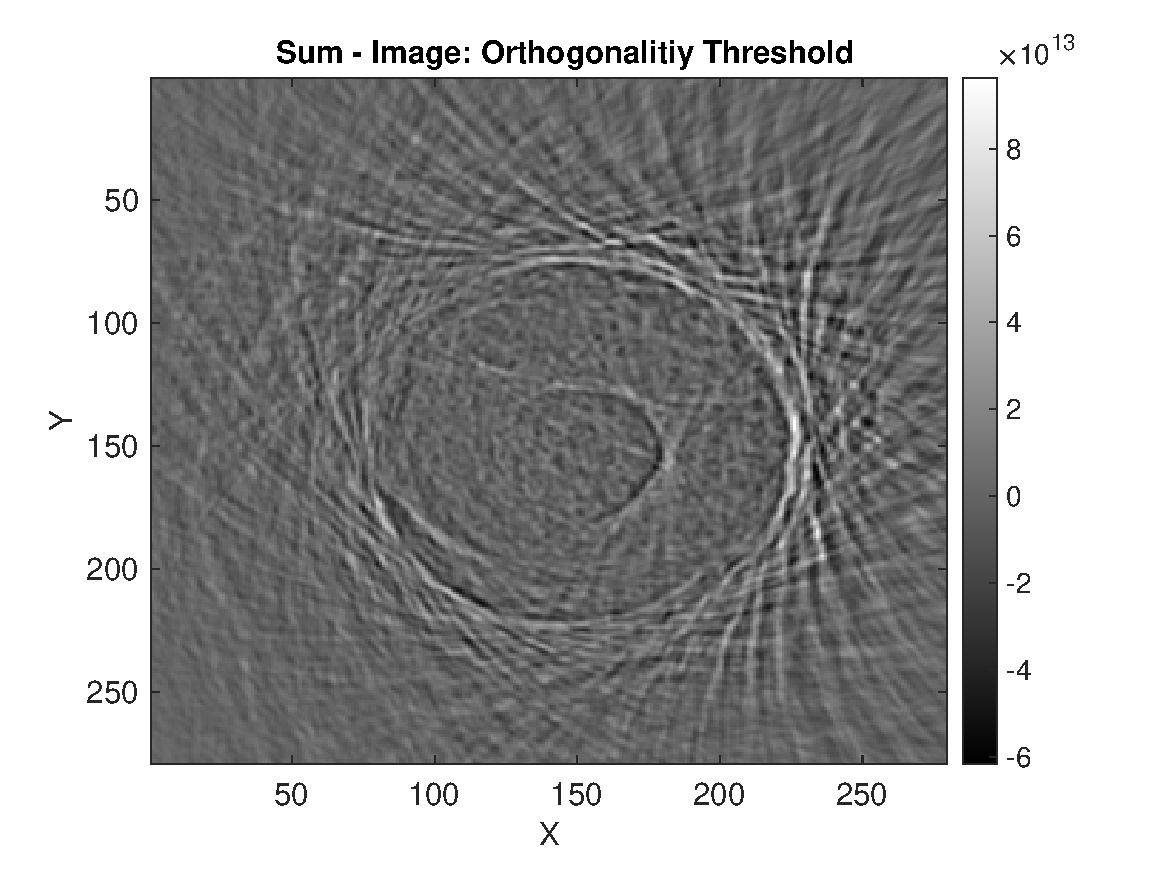
\includegraphics[width=1.12\textwidth,right]{Graphics/Results/Diff_angle_sort_orthogonality/diff_ortho_bubble_sumImmage_sort.eps}
         \caption{Angle Sorting method.}
         \label{fig:res:summareized_bubble_ortho_image_bubble}
     \end{subfigure}
        \caption{Summarised image where the 4D image was reduced to a 3D image. }
        \label{fig:res:summareized_bubble_ortho_image}
\end{figure}

Again the 166th slice in the z-direction is shown. In comparison to Figure \ref{fig:res:slice_diff_bubble_ortho_image} the olive in the middle of the volume become much more prominent. The olive was evenly irradiated by the ultrasound waves by all emitter around the test object. In the image of only one direction vector the olive showed a high intensity of sound waves in the top right corner of the olive. With the summation of all the images now this information is lost. Again the Angle Sorting algorithm yielded the image with the higher contrast. Still, both images contain enough information to make out the olive and the stone in the middle. The difference between the two summarised images from Figure \ref{fig:res:summareized_bubble_ortho_image} is shown next:

\begin{figure}[H]
    \centering
    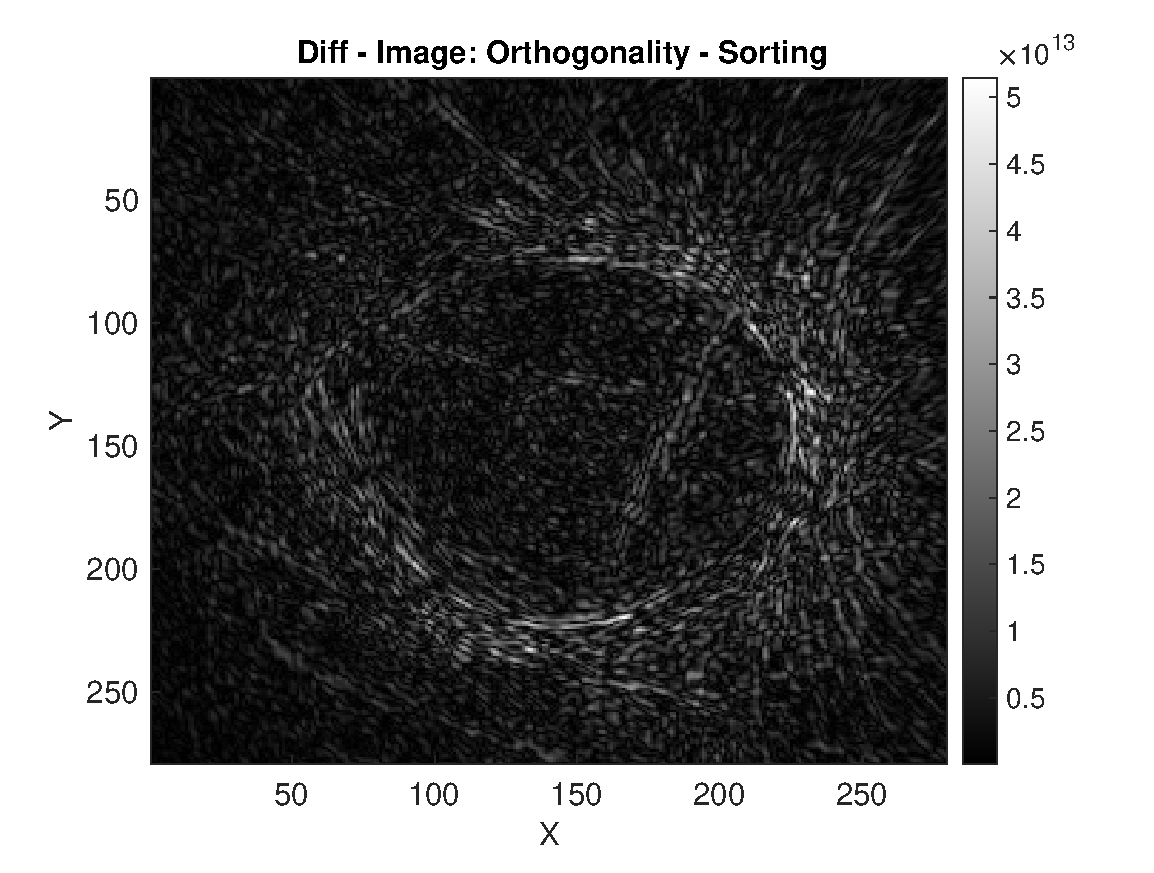
\includegraphics[width=0.82\linewidth]{Graphics/Results/Diff_angle_sort_orthogonality/diff_ortho_bubble_diffimage.eps}
    \caption{Absolute value of the difference between the summarised image of the Orthogonality Method and the Angle Sorting method. }
    \label{fig:diff_image}
\end{figure}

The biggest differences can be found on the outer boundary of the olive where many reflections took place. The are inside of the olive and the rest of the measurement volume are less influenced by the new method. 




\section{Input Data and representation}
The test data that was used during this thesis mainly was part of the data set '$exp0040\_Carina\_PhantomGelatineOlive\_mitHalterung$'. For this data an olive inside a gelatin block was examined in the \ac{usct}. The \acp{ascan} were recorded for all 157 \ac{tas} with ten aperture rotation positions so a total of $157\cdot4\cdot157\cdot9\cdot10 = 8.8\cdot10^6$ \acp{ascan} were recorded. The reconstructed reflection image for this data set is shown in Figure \ref{fig:res:reflec_image_olive_xyz}. The sub plots each show a slice through the image. The coloured lines in each plot show the selected slice in the other two coordinate systems. The blue marker belongs to the z-dimension, the green one corresponds to the y-dimension and therefore the red marker shows the x-dimension. Figure \ref{fig:res:reflec_image_olive_xyz_x} shows the x-layer for $x = 0$. That x is equal to zero can be seen in the other two figures where the red markers are located at about 0. Analogously, Figure \ref{fig:res:reflec_image_olive_xyz_y} and  \ref{fig:res:reflec_image_olive_xyz_z} show the y-layer and z-layer of the image.

\begin{figure}[H]
     \centering
     \begin{subfigure}[b]{0.49\textwidth}
         \centering
        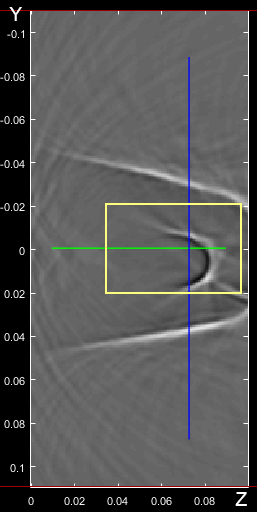
\includegraphics[width=0.59\linewidth]{Graphics/Results/Olive_Standart_reco_example/olive_standart_reconstruction_whole_volume_x_layer.png}
         \caption{x-Layer}
         \label{fig:res:reflec_image_olive_xyz_x}
     \end{subfigure}
     \hfill
     \begin{subfigure}[b]{0.49\textwidth}
         \centering
         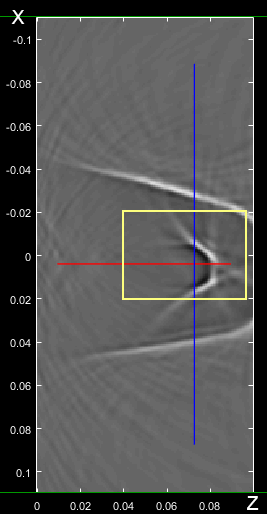
\includegraphics[width=0.61\textwidth]{Graphics/Results/Olive_Standart_reco_example/olive_standart_reconstruction_whole_volume_y_layer.png}
         \caption{y-Layer}
         \label{fig:res:reflec_image_olive_xyz_y}
     \end{subfigure}
     \hfill
     \begin{subfigure}[b]{0.55\textwidth}
         \centering
         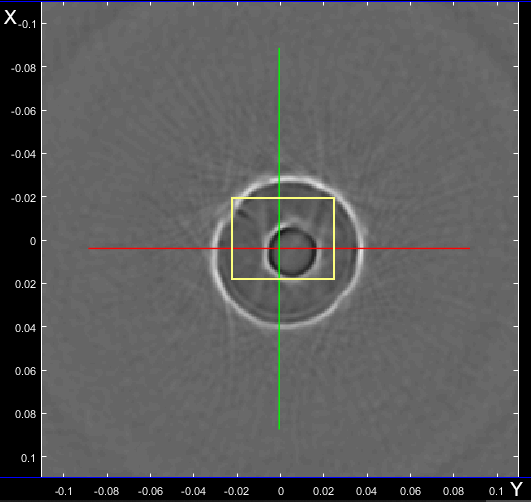
\includegraphics[width=0.99\textwidth]{Graphics/Results/Olive_Standart_reco_example/olive_standart_reconstruction_whole_volume_z_layer.png}
         \caption{z-Layer}
         \label{fig:res:reflec_image_olive_xyz_z}
     \end{subfigure}
        \caption{Reconstructed reflection image of an olive in gelatin. The yellow box markes the area that was used during the reconstructions with five dimension to limit the amount of data.
        Name of the data set: '$exp0040\_Carina\_PhantomGelatineOlive\_mitHalterung$'.}
        \label{fig:res:reflec_image_olive_xyz}
\end{figure}

The volume was only partially considered during the reconstruction to reduce the amount of data that had to be processed and with that reduce the computation time. The start point for the volume was set to $[\, -0.02,\, -0.02,\, 0.04\, ]$ and the end point was set to: $[ 0.02,\, 0.02,\, 0.095\, ]$. The utilised area is marked with the yellow boxes in Figure \ref{fig:res:reflec_image_olive_xyz}. The marked volume was chosen to be as central on the olive as possible. Three different tissue samples are included in this data set: the stone in the middle of the olive, the flesh of the olive as well as the outer shell of the olive. 
      
      
\section{Influence of \ac{sos} Correction }

\section{Resolution of the segmentation}


\section{Demultiplexing of image index in the CUDA-Kernel}
\label{demultiplexing_structure}




\section{Performance of the index identification methods}
\label{performance_index_ident}

In Section \ref{sec:index_ident} two main approaches were presented for the assignment of the direction vector index to each \ac{ascan}. In this chapter the results of the performance evaluation of the angle sorting approach from section \ref{chap:angle_sorting} and the threshold orthogonality from section \ref{chap:ortho_threshold} are shown. For each implementation of the assigning method the calculations of the reconstruction volume were done separately. All the following executions were performed on two \acp{gpu} with a reconstruction volume of 279x279x233 voxels. Furthermore, only the first 30235 \acp{ascan} were used during the reconstruction to speed up the process. The four dimensional case was considered and therefore only the comparison vector from the voxel to the receiver was used. No results besides the profiling report were saved to minimise the influence of hard drive operations during the performance evaluation. The execution time includes all initialisation steps of the reconstruction algorithm as well as generation of direction vectors and calculation of the fringe orthogonality (in case of the application of the orthogonality threshold method). For each data point in the following graphs the reconstruction function was called in a looping manner depending on the number of direction vectors that are used as input for the algorithm following the flow chart of Figure \ref{Basic_Algo_Angle_ident}. The first reconstruction was started for 14 direction vectors and the last ended at 126. The reason for staring at 14 is that below that the direction vectors were generated with the help of platonic solids and could not be increased as freely as with the arbitrary segmentation approach.

The following three figures shows the comparison of the computation time of the different techniques for the index identification introduced in Section \ref{sec:index_ident}. The results for the sorting algorithm are presented in blue as the approach with the orthogonality threshold is shown in red.

\begin{figure}[H]
    \centering
    \fbox{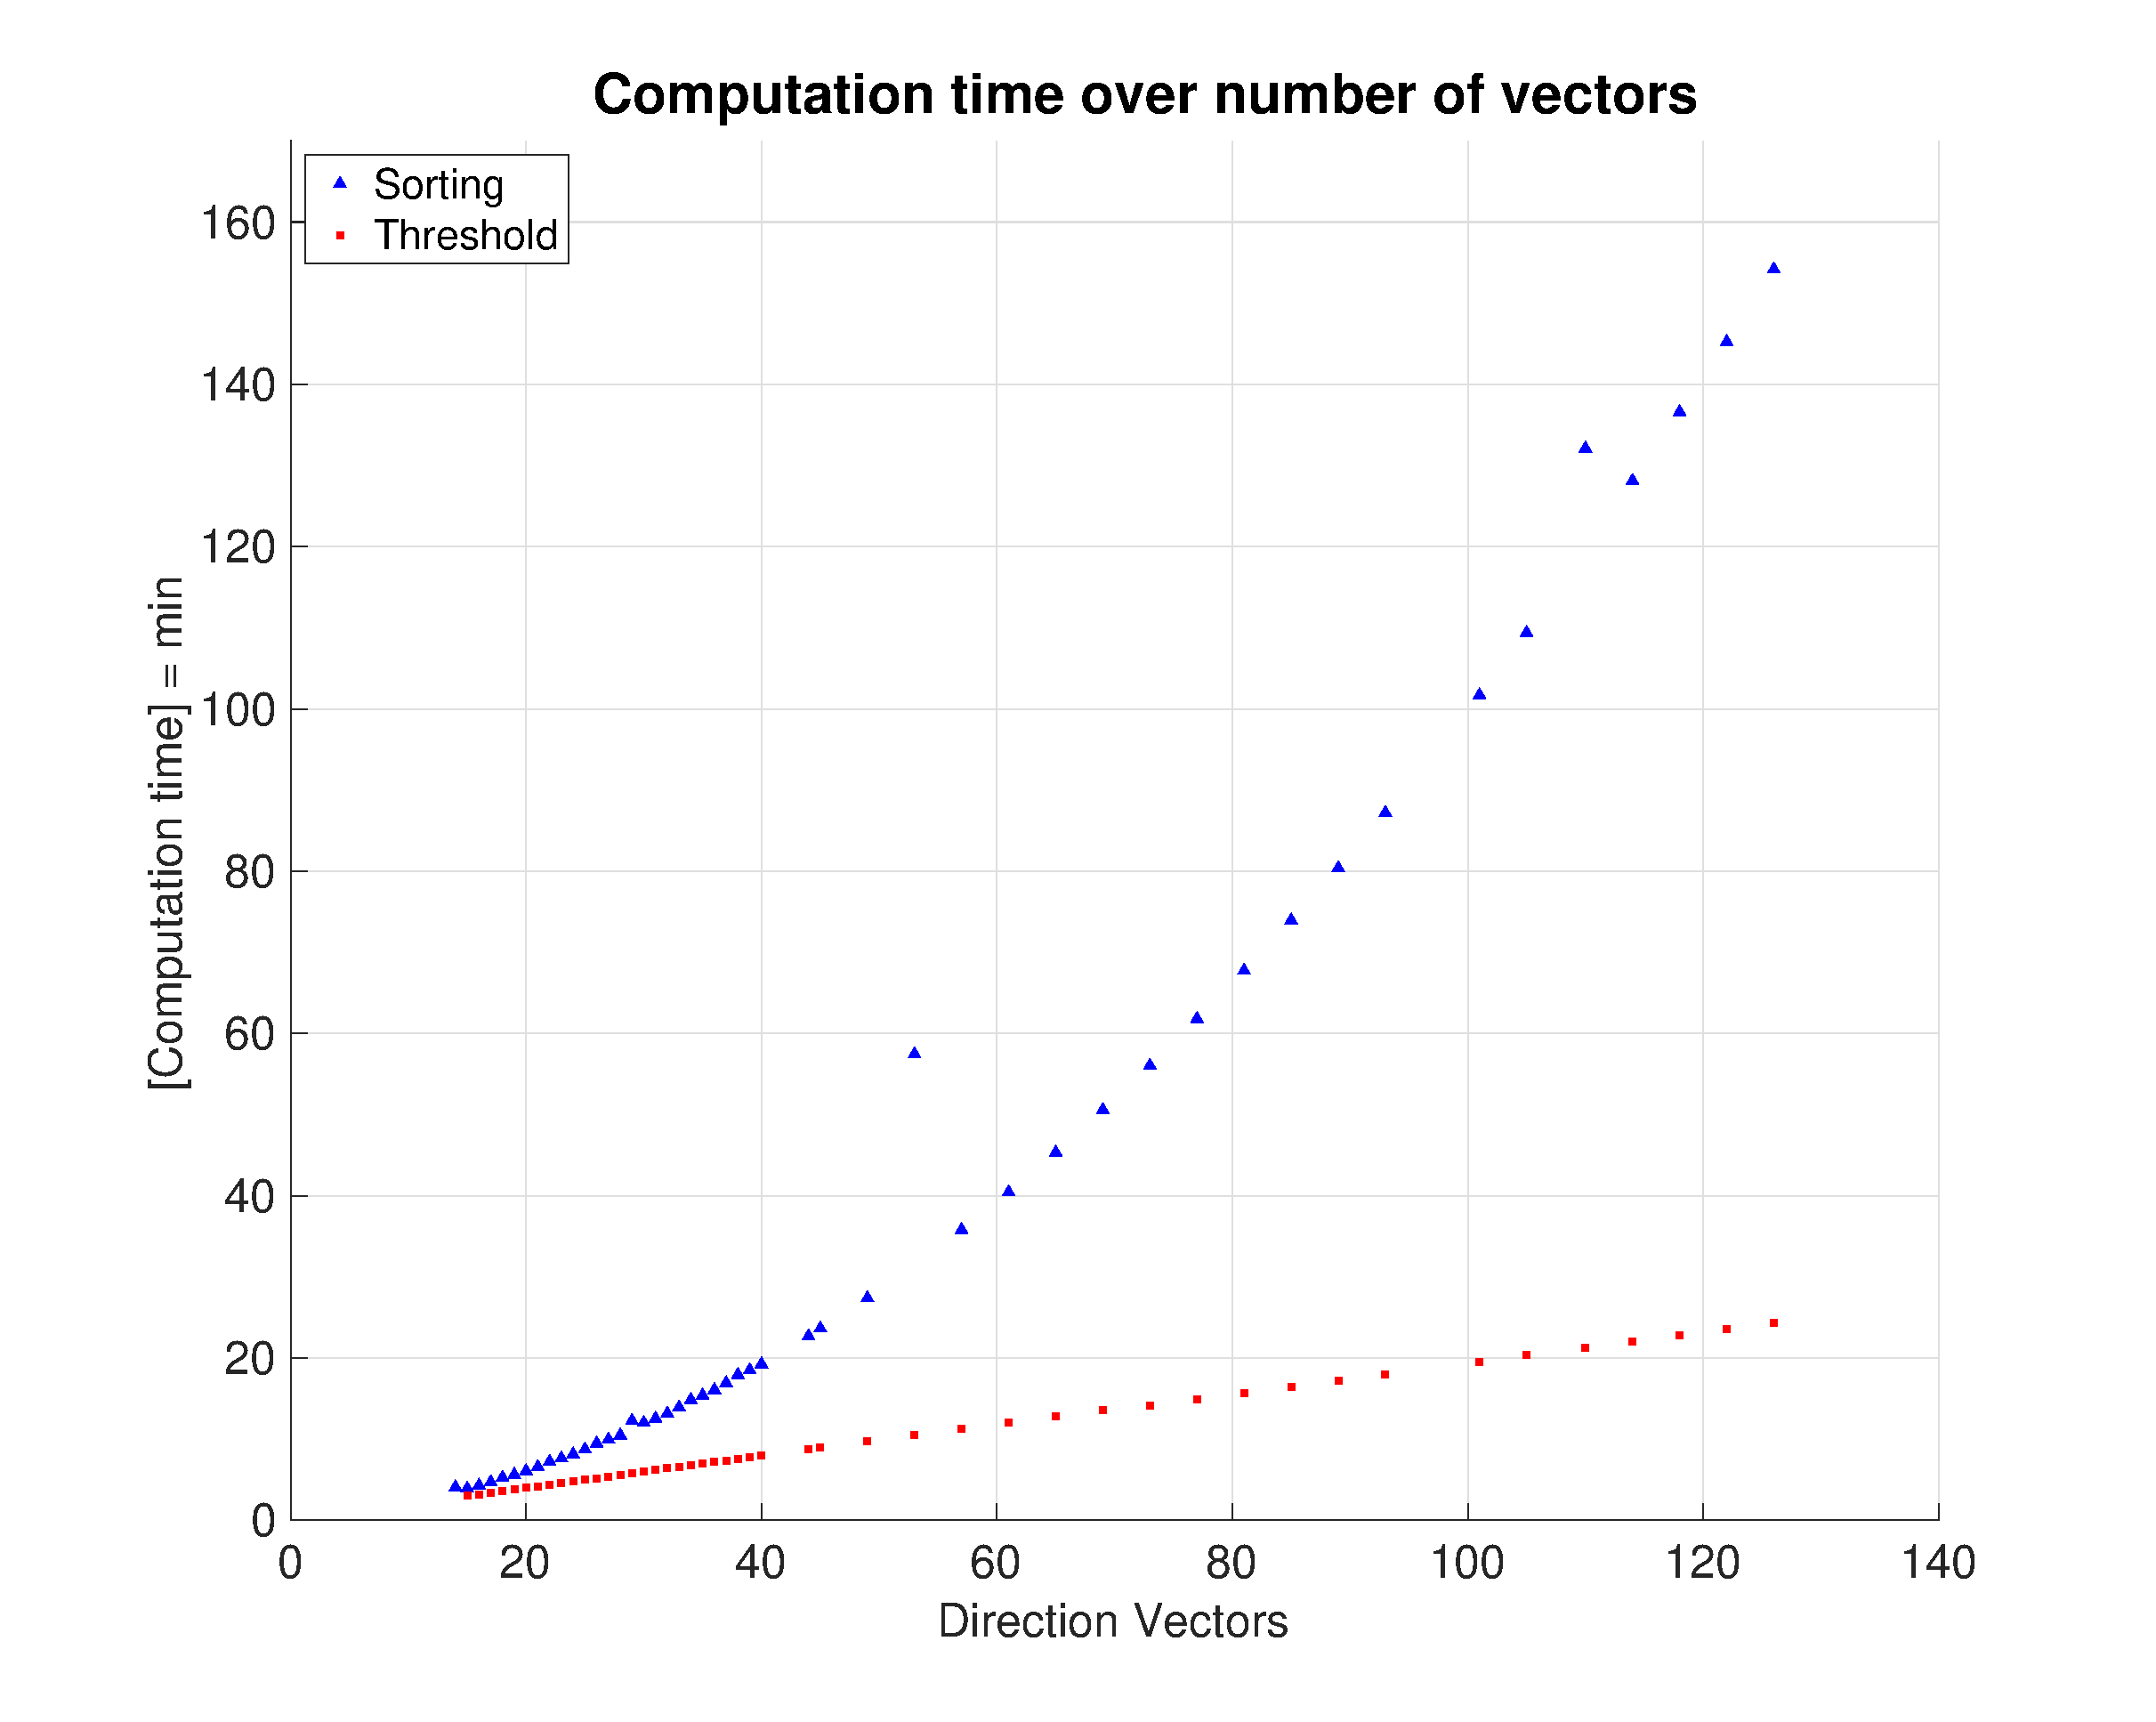
\includegraphics[width=0.76\linewidth]{Graphics/Results/complete_computation_time_over_numer_vec.eps}}
    \caption{Total time of computation given in minutes for 30325 \acp{ascan} and for all loops over the direction vectors. The red markers represent the execution time for the orthogonality threshold method. The blue markers belong to the angle sorting algorithm.}
    \label{fig:Complete_computation_all_vecs}
\end{figure}

The blue triangle markers in Figure \ref{fig:Complete_computation_all_vecs} represent the execution time for the angle sorting algorithm. The horizontal distances between the succeeding markers is associated with the attempt to decrease the overall length of the experiment. For shorter execution times (up to 20 minutes per call) for both algorithms the amount of direction vectors were increased one by one after each iteration. The following steps were increased by four input vectors per iteration.

For a small number of direction vectors the execution time of the angle sorting algorithm and the orthogonality threshold are relatively close, both taking approximately three minutes to compute. With increasing number of direction vectors the application of the angle sorting algorithm leads to a longer sorting loop. This can be seen in the exponential growth of the execution time for the implementation of the angle sorting method. In contrast the implementation of the orthogonality threshold method shows a linear behaviour when the number of direction vectors is increased. For the final 126 direction vectors the sorting algorithm takes $154 \min$ whereas the orthogonality method takes $24,3 \min$ to finish, thus being $10,5$ times higher than the faster orthogonality method. For 45 direction vectors the reconstruction with the angle sorting method takes $23,6 \min$ and thus approximately as long as the orthogonality method takes with 126 direction vectors.

The execution times of each iteration and number of direction vectors include a significant amount of overhead, as it was mentioned further above. Since the overhead is expected to be constant for every execution of the reconstruction algorithm. Regardless of the overhead these results still show the considerable influence of the assigning algorithm on the overall performance.

During the performance evaluation certain iterations took an unusual amount of time to finish and led to some outliers in the computation time for the sorting algorithm. Those were non-reproducible for the particular number of direction vectors for when they occurred but were kept in the graph for reasons of consistency. One possible explanation might be the accidental use of the same  \acp{gpu} by another process or other occurrences that might have led to the simultaneous occupation of servers resource and thus a decreased performance of the reconstruction algorithm since multiple people have access to it.


\begin{figure}[H]
    \centering
    \fbox{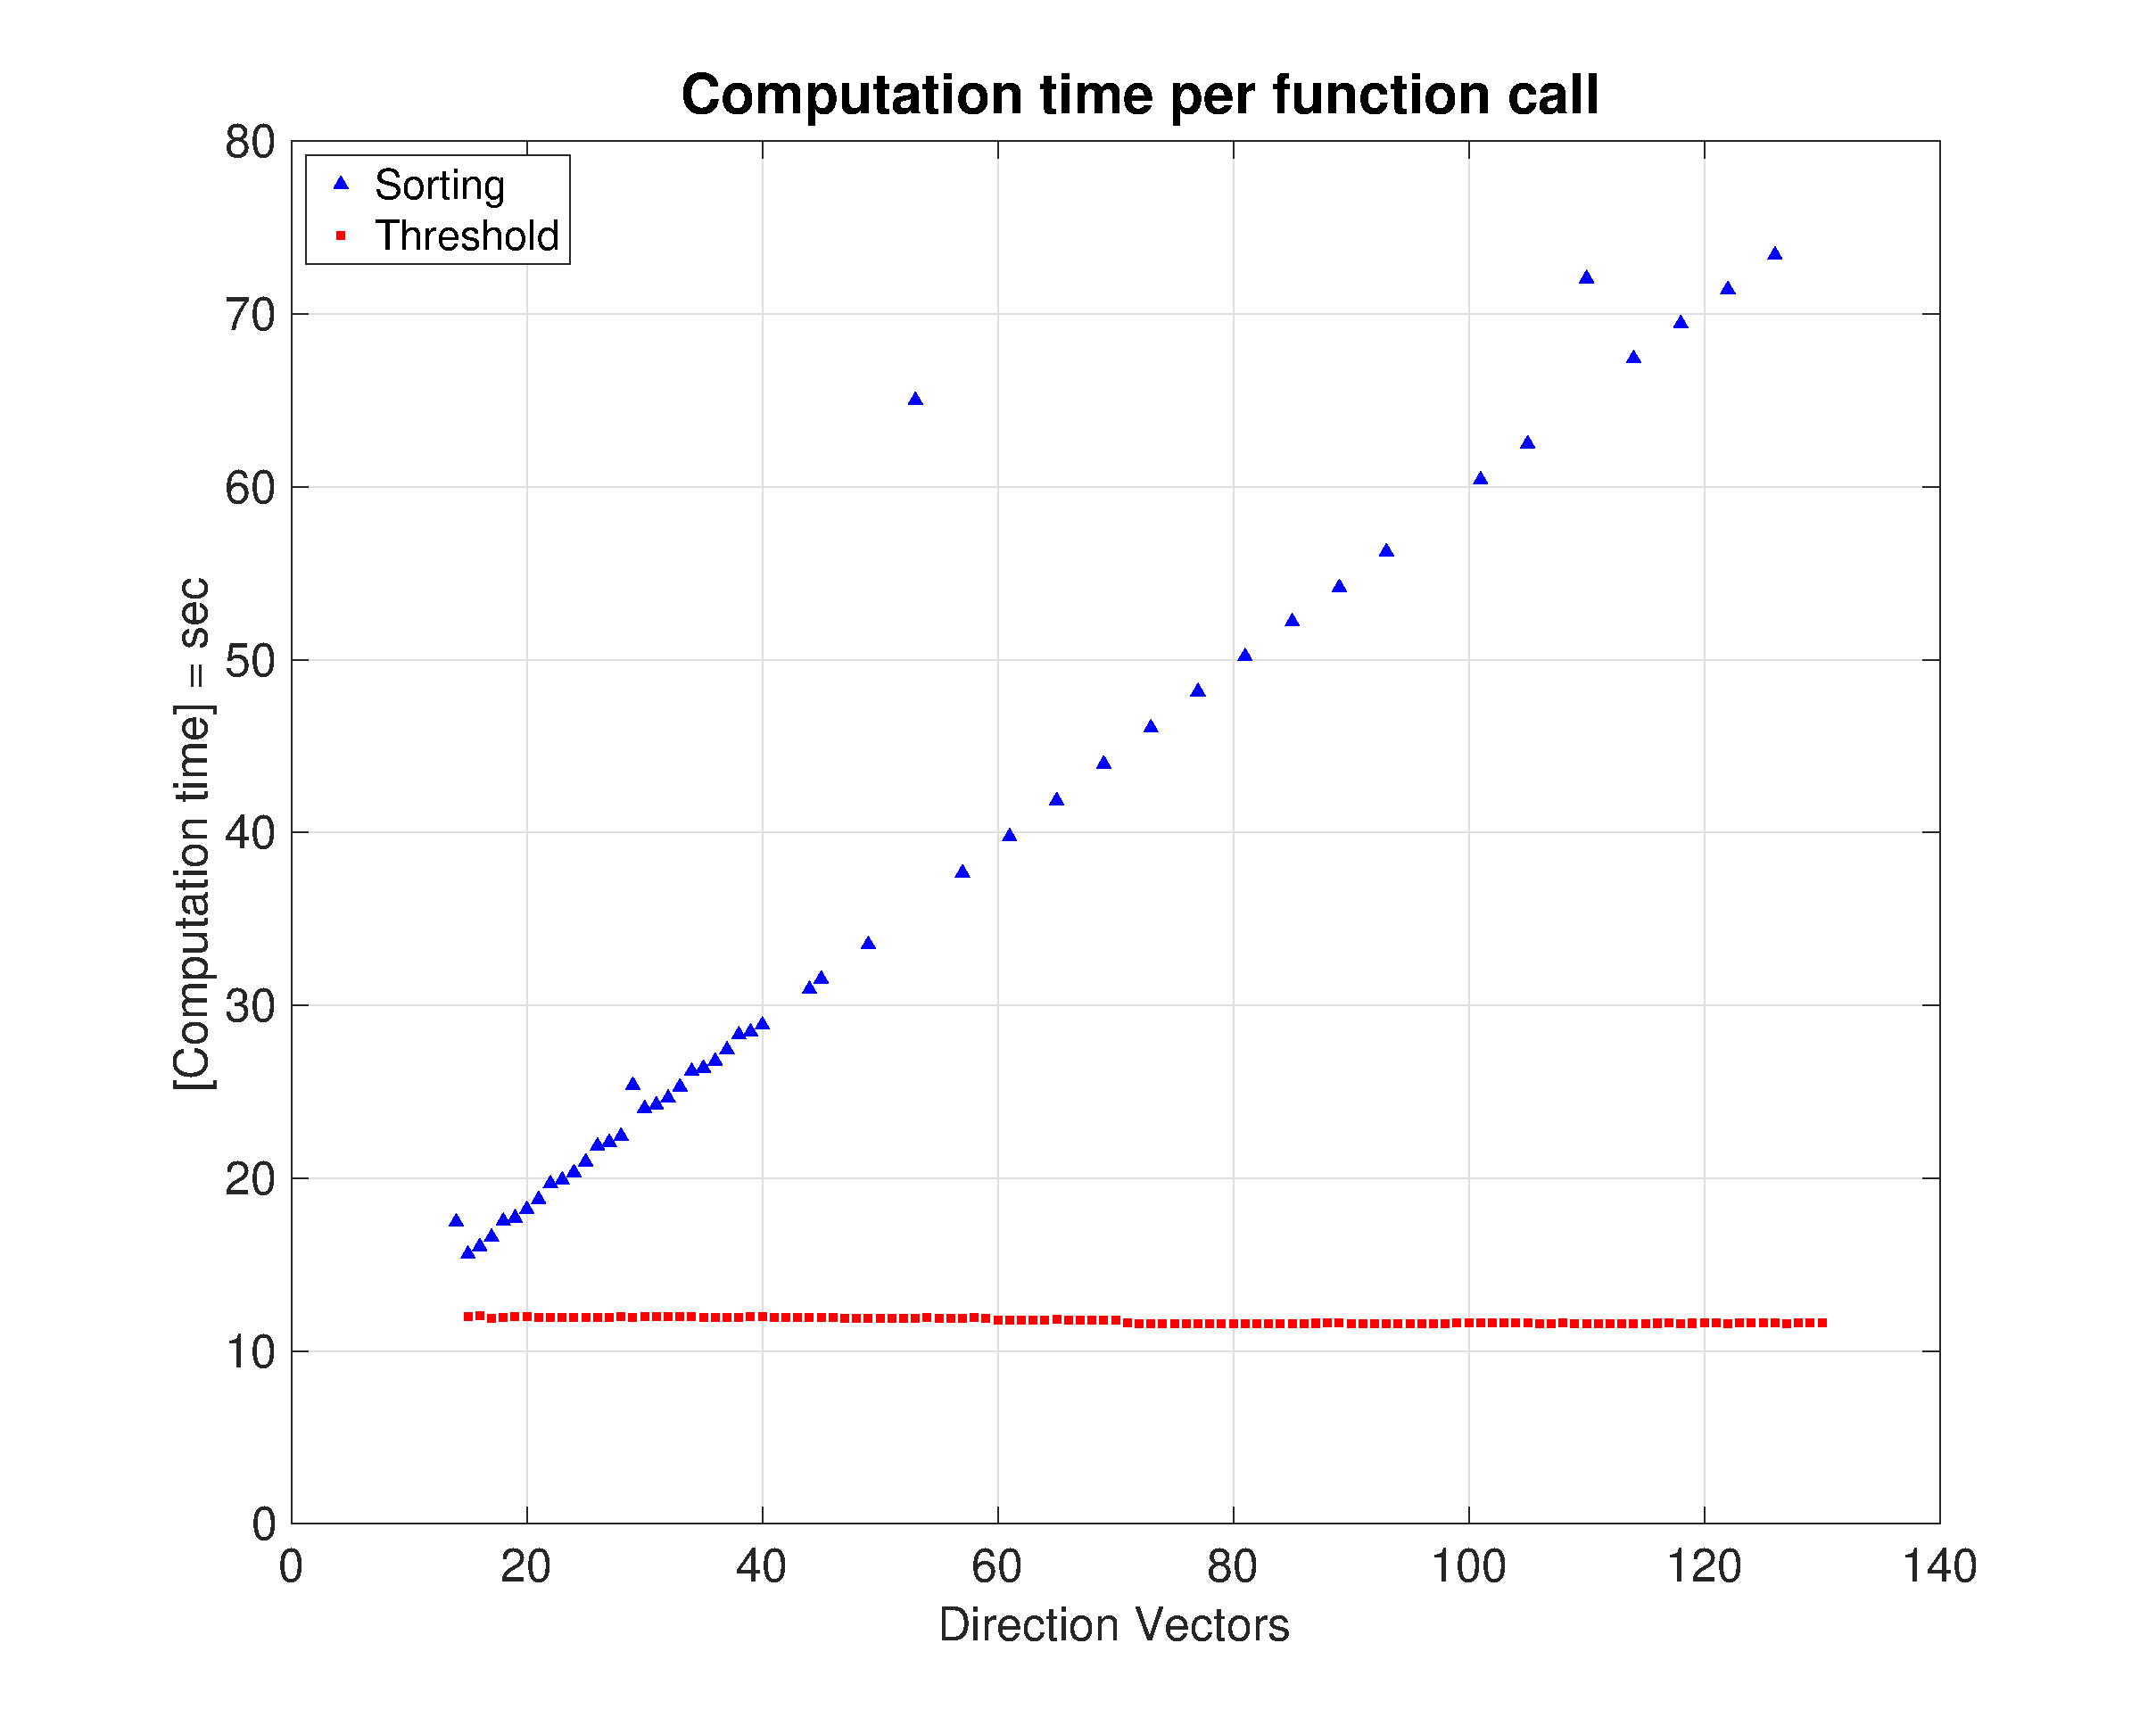
\includegraphics[width=0.76\textwidth]{Graphics/Results/computation_time_per_mexcall.eps}}
    \caption{The computation time of each individual function call in $\sec$. The complete execution time was divided by the   }
    \label{fig:computation_per_mex}
\end{figure}

In Figure \ref{fig:computation_per_mex} the execution time for only one iteration of the reconstruction is shown. The complete computation time was divided by the number of input direction vectors to approximate the execution duration for only one function call. The resulting plot shows that the execution time for the orthogonality threshold method is rather constant for an increasing number of direction vectors. In contrast the execution time for each function call with the implementation of the sorting algorithm takes an increasing amount of time to finish. The outliers in the set of blue markers are visible again in this plot. The red markers for the threshold method seem to have a step at about 70 input vectors. The reason for that most likely is the different time of day when the executions were started. They were not done consecutively but sometimes had to be restarted at a later point. This also was the case for the performance analysis for the threshold method. Beginning with 70 input direction vectors the profiling script was restarted the day after. The reason for the small difference in execution time again might be found in the shared resources on the server and the non-constant load during the calculations. 



\begin{figure}[H]
    \centering
    \fbox{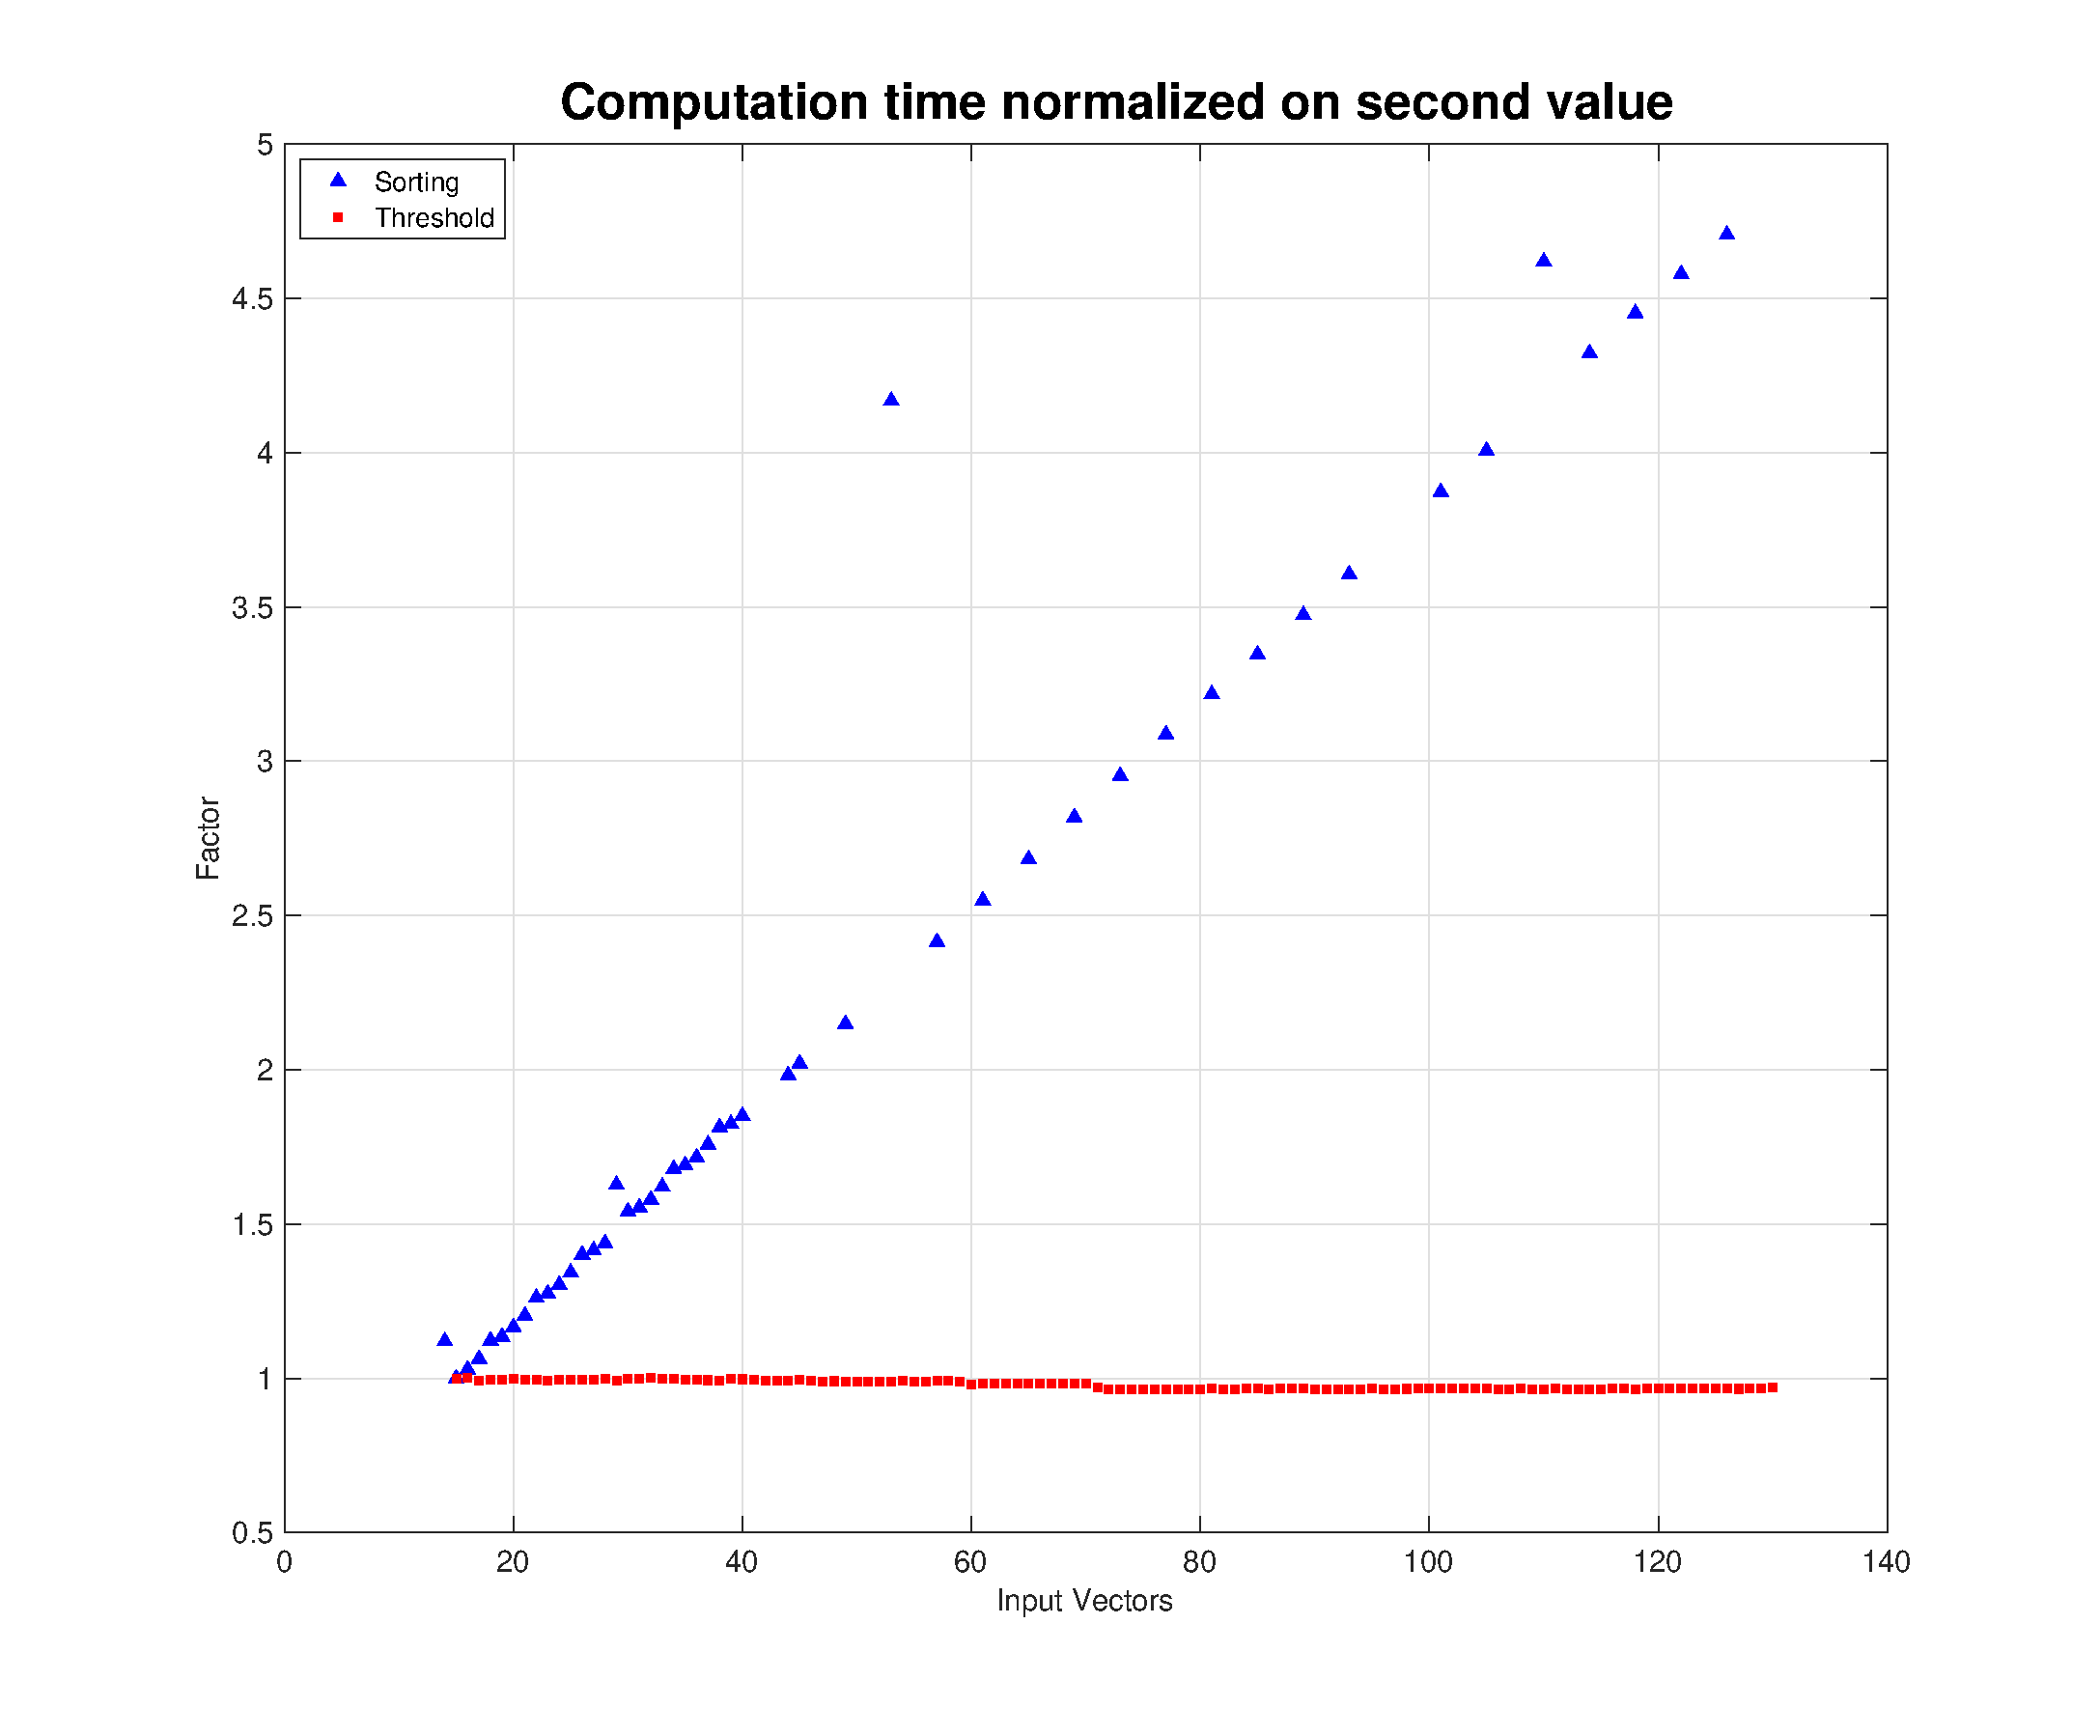
\includegraphics[width=0.76\textwidth]{Graphics/Results/computation_normlaized_2nd_value.eps}}
    \caption{The computation time of each individual function call was normalised on the 2nd value of both methods.}
    \label{fig:computation_normlaized_2nd}
\end{figure}

To quantify the differences in performance between both approaches in Figure \ref{fig:computation_normlaized_2nd} the execution times for both methods were normalised on their respective second value. The second value was preferred over the first one since the first iteration always took a bit longer than the following one. A reason for that might be initial behaviour of the servers processing uni e.g. the optimisation of the cache management at the beginning of the calculations. Nevertheless, in bath cases the markers for 14 direction vectors begin at the factor 1 and increase over the following iterations with more input vectors. At least this is the case for the angle sorting method. The markers for the orthogonality threshold stay rather constant at 1 whereas the blue markers end up at a factor of $4.706$ for 126 input vectors. Here again the small step around the 70 input vectors arise from the different times of the start of the analysis.

